\setcounter{chapter}{4}

\chapter{导数的应用}

微分学最初是独立于积分学的,因为其自身已经可以解决许多的应用问题。
本章讨论的极值、最值、单调性和曲率等,都是微分学的独立应用,其中
中值定理和Taylor公式又可以说是整个微分学的“制高点”,集成和融汇
了导数与微分的绝大部分思想与概念,正确地理解和熟练掌握这部分的知识
是对微积分有一个全面深刻认识的基础。

% \begin{shaded}
% 	{\bf 多项式函数的拐点、极值点的判定:}设
% 	$$P(x)=(x-a_1)^{k_1}(x-a_2)^{k_2}\ldots(x-a_n)^{k_n},$$
% 	其中$a_i\in\mathbb{R}(i=1,2,\ldots,n)$(称为$P(x)$的{\it 零点},
% 	或$P(x)=0$的{\it 根}),$k_i\in\mathbb{Z}^+(i=1,2,\ldots,n)$
% 	(称为$a_i$对应的{\it 重数})。如下准则成立:
% 	\begin{itemize}
% %   	  \setlength{\itemindent}{1cm}
% 	  \item {\bf 所有二次以上的重根均为驻点,其中偶数次的为极值点,奇数次的为拐点}
% 	  \item {\bf 两个相邻零点之间有且仅有一个极值点}
% 	  \item {\bf 两个相邻驻点之间有且仅有一个拐点}
% 	\end{itemize}
% 
% 	{\bf 例:}$y=(x-1)(x-2)^2(x-3)^3$有几个极值点和拐点?
% 
% 	{\bf 解:}利用前述的判定准则:
% 	\begin{enumerate}[(1)]
%   	  \setlength{\itemindent}{1cm}
% 	  \item $x=2$为$2$重根,故为驻点兼极值点
% 	  \item $x=3$为$3$重根,故为驻点兼拐点
% 	  \item 在$(1,2)$和$(2,3)$中各有一个驻点兼极值点,记为$\xi_1,\xi_2$
% 	  \item $4$个驻点由小到大的排列为
% 	  $$\xi_1<2<\xi_2<3,$$
% 	  故在其间有且仅有$3$个拐点
% 	\end{enumerate}
% 
% 	综上,该函数共有$3$个极值点,$4$个拐点。
% 
% 	{\bf 例:}$y=2(x+1)^5(x-2)^8(x-4)^3+9$有几个极值点和拐点?
% 
% 	{\bf 解:}注意到该函数和
% 	$$y=2(x+1)^5(x-2)^8(x-4)^3,$$
% 	的极值点和拐点完全相同,故我们只需研究后者的极值点和拐点个数:
% 	\begin{enumerate}[(1)]
%   	  \setlength{\itemindent}{1cm}
% 	  \item $x=-1$为$5$重根,故为驻点兼拐点
% 	  \item $x=2$为$8$重根,故为驻点兼极值点
% 	  \item $x=4$为$3$重根,故为驻点兼拐点
% 	  \item 在$(-1,2)$和$(2,4)$中各有一个驻点兼极值点,记为$\xi_1,\xi_2$
% 	  \item $5$个驻点由小到大的排列为
% 	  $$-1<\xi_1<2<\xi_2<4,$$
% 	  故在其间有且仅有$4$个拐点
% 	\end{enumerate}
% 
% 	综上,该函数共有$3$个极值点,$6$个拐点。
% 
% \end{shaded}

\section{函数的极值与最值}

{\bf 问题:}给定一个函数,如何求其最大和最小值?

{\bf 教材-例1:}画出函数$f(x)=3x^4-4x^3-12x^2+3$在区间$[-2,3]$,通过
观察求其最大和最小值。

\begin{center}
	\resizebox{!}{5cm}{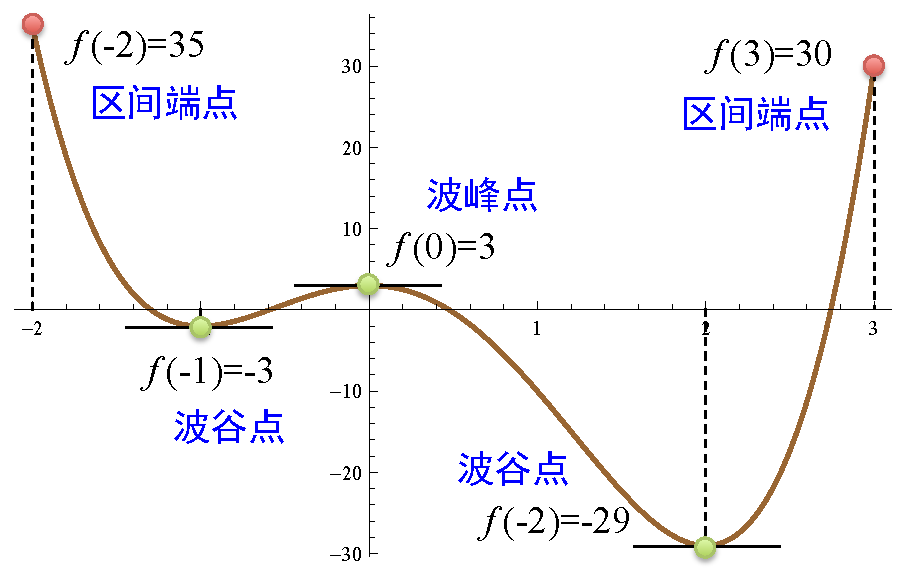
\includegraphics{./images/ch5/fmm_pt.pdf}}
\end{center}
\vspace{-2em}
$$f(-2)=35,\quad f(3)=30,\quad f(2)=-29$$

{\bf 定理5.1.1}(Fermat引理):若函数$f(x)$在$x_0$处可导,且在$x_0$的某邻域内,有
$$f(x)\geq f(x_0)\quad (\mbox{或}\quad f(x)\leq f(x_0))$$
则$f'(x_0)=0$。\ps{掌握费马引理的证明方法}

\begin{shaded}
	{\bf 关于Fermat和Fermat's Last Theorem}
	
	Pierre de Fermat(1601-1665),法国律师和业余数学家。
	他在数学上的成就不比职业数学家差,他似乎对数论最有兴趣,亦对现代微积分的建立有所贡献。
	\begin{itemize}
	  \item 微积分:{\it 费马引理}
	  \item 将阿波罗尼奥斯的几何分析中用代数方法来重新建立,开出{\it 解析几何}之路。
	  (费马只使用一轴,只接受正数的答案。后世多以笛卡尔为解析几何的创立者,
	  主因是费马没有发表其作品。)
	  \item 1654年,和Pascal在书信中的讨论,被认为是{\it 概率论}的开端,
	  1656年和概率论的正式创立者Christiaan Huygens(1629-1695)的交流,
	  使后者增加了对概率论的兴趣
	\end{itemize}
	
	Fermat{\it 小定理}:假设$a\in\mathbb{Z}$,$p$为素数,则$a^p-a$可以整除$p$,
	或者写为
	$$a^p\equiv a(\mathrm{mod}p),$$
	特别低,若$a$不是$p$的倍数,则上式可写为$a^{p-1}\equiv 1(\mathrm{mod} p)$
	
	Fermat{\it 大定理}(也称Fermat最后定理):对于大于$2$的正整数$n$,以下方程
	无正整数解
	$$x^n+y^n=z^n.$$
	这个定理造成了数学史上最大的悬案:1637年,费马在阅读丢番图《算术》拉丁文译本时,
	曾在第11卷第8命题旁写道:
	{\it 将一个立方数分成两个立方数之和,或一个四次幂分成两个四次幂之和,
	或者一般地将一个高于二次的幂分成两个同次幂之和,这是不可能的。
	关于此,我确信已发现了一种美妙的证法,可惜这里空白的地方太小,写不下。}
	
	一直被称为“费马猜想”,直到英国数学家Andrew John Wiles及其学生Richard
	Taylor于1995年将他们的证明出版后,才称为“费马大定理”。
	经过数学家们三个多世纪的努力,猜想才变成了定理。在冲击这个数论世纪难题的过程中,
	无论是不完全的还是最后完整的证明,都给数学界带来很大的影响;很多的数学结果、
	甚至数学分支在这个过程中诞生了,包括代数几何中的{\it 椭圆曲线}和{\it 模形式},
	以及{\it	伽罗瓦理论}和{\it 赫克代数}等。这也令人怀疑
	当初费马是否真的找到了正确证明。
	
	\begin{itemize}
	  \item 1770年,Euler证明 $n=3$时定理成立
	  \item 1823年,Legendre证明$n=5$时定理成立
      \item 1832年,Dirichlet试图证明$n=7$失败,但证明$n=14$时定理成立
	  \item 1839年,Gabriel Lamé证明$n=7$时定理成立
	  \item 1850年,Ernst Eduard Kummer证明$2<n<100$时除$37$、$59$、$67$三数外定理成立
	  \item 1955年,Harry Vandiver以电脑计算证明了对所有不超过$2521$的素数定理成立
	  \item 1976年,Samuel Wagstaff以电脑计算证明对所有不超过$125000$的素数定理成立
	  \item 1985年,电脑计算证明了对所有小于$4$百万的素数定理成立
	  \item 1987年,格朗维尔以电脑计算证明了$2<n<10^{{1800000}}$时定理成立
	  \item 1995年,Wiles证明$n>2$时定理成立。
	\end{itemize}
	
	怀尔斯证明费马大定理的过程亦甚具戏剧性。他用了七年时间,在不为人知的情况下,
	得出了证明的大部分;然后于1993年6月在一个学术会议上宣布了他的证明,并瞬即
	成为世界头条。但在审批证明的过程中,专家发现了一个极严重的错误。怀尔斯和泰勒
	然后用了近一年时间尝试补救,终在1994年9月以一个之前怀尔斯抛弃过的方法得到成功。
	
	为什么Fermat大定理在数学史上的地位如此重要?有三个主要的原因:一是问题基本,长时间
	(350年)悬而未决,吸引了众多数学大师对其加以研究;二是研究问题的过程中产生了新的思想和方法,
	带动了数学很多领域的发展;三是涉及{\it 谷山—志村猜想},是现代数学大热门{\it 朗兰兹纲领}
	的重要组成部分。1967年提出的朗兰兹纲领(Langlands program)指出三个
	相对独立发展起来的数学分支	:数论、代数几何和群表示论,实际上是密切相关的,
	而连接这些数学分支的纽带是一些特别的函数,被称为L-函数。L-函数可以说是朗兰兹纲
	领的中心研究对象。数学界著名的七个	{\it “千禧年大奖问题”}中有两个就是关
	于L-函数的,它们分别是{\it 黎曼假设}和{\it BSD猜想}。
	
	延伸阅读:
	
	[1] 知乎:为什么费马大定理在数学史上的地位如此重要?
	
	[2] 知乎:为什么费马大定理表述起来这么简单,证明却这么复杂?
	
	[3] https://en.wikipedia.org/wiki/Fermat's\_Last\_Theorem
	
	[4] https://zh.wikipedia.org/wiki/费马大定理
	
	[5] https://en.wikipedia.org/wiki/Andrew\_Wiles
	
	[6] https://en.wikipedia.org/wiki/Pierre\_de\_Fermat
	
\end{shaded}

\subsection{极值}

{\bf 定义5.1.1:}\ps{极值即{\b 局部唯一的最值}}设在$x_0$的某去心邻域内,恒有
$$f(x)<f(x_0)\quad (\mbox{或}\quad f(x)>f(x_0)),$$
则称$f(x_0)$是$f(x)$的一个{\it 极大(小)值},$x_0$称为$f(x)$的一个{\it 极值点}。

\begin{itemize}
  \setlength{\itemindent}{1cm}
  \item {\b 函数在极值点处未必可导} 
  \item {\b 可导函数极值点处的导数为零} 
  \item {\b 导数为零的点({\it 驻点})未必是极值点}
\end{itemize}

\begin{center}
	\resizebox{!}{4cm}{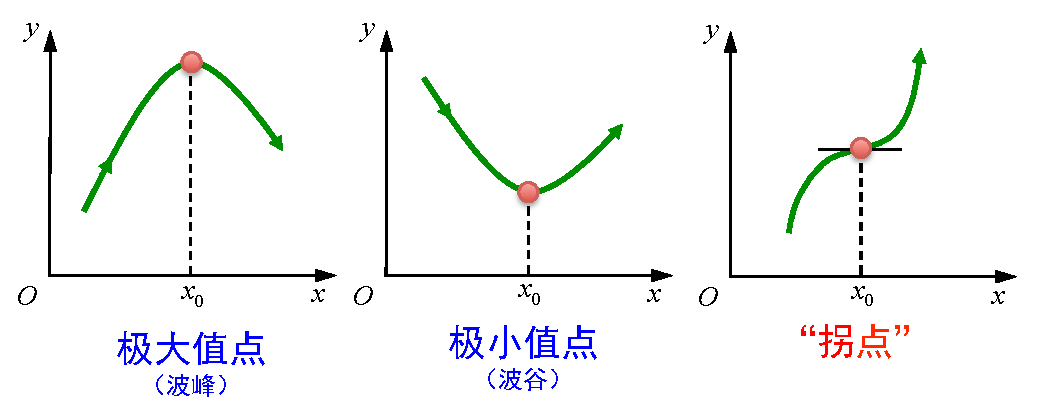
\includegraphics{./images/ch5/edge_pt.pdf}}
\end{center}

{\bf 定理5.1.2}(极值判定的充分条件)设$f(x)$在$x_0$附近连续,
若$f(x)$在$x_0$两侧单调性发生改变,则$f(x)$在$x_0$取极值。\ps{这个条件是充要的吗?}

{\bf 注:}{\b 连续函数单调性的分界点是函数的极值点。}

{\bf 例:}判断正误
\begin{enumerate}[(1)]
  \setlength{\itemindent}{1cm}
  \item {\b 函数的极大值一定是最大值\quad  ({$\times$})} 
  \item {\b 函数的最大值一定是极大值\quad  ({$\times$})} 
  \item {\b 函数的极大值一定比极小值大\quad  ({$\times$})} 
\end{enumerate}

\subsection{最值(最优化)问题}

{\bf 问:}在闭区间上,函数可能在什么位置取到最值?

\begin{center}
	\resizebox{!}{4cm}{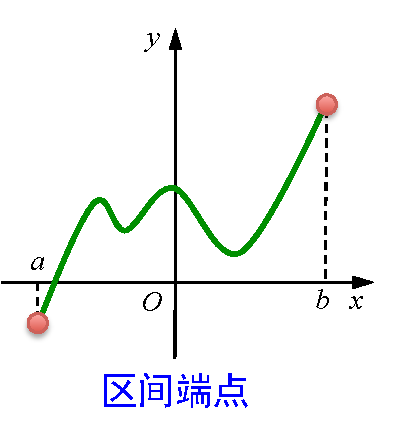
\includegraphics{./images/ch5/mm1.pdf}}
	\resizebox{!}{4cm}{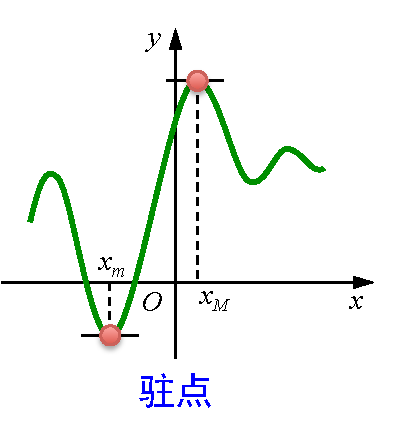
\includegraphics{./images/ch5/mm2.pdf}}
	\resizebox{!}{4cm}{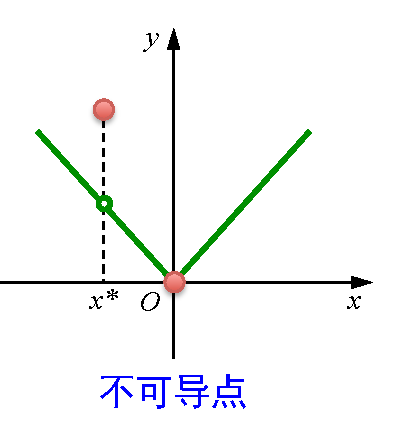
\includegraphics{./images/ch5/mm3.pdf}}
\end{center}

{\bf 求闭区间上连续函数的最值:}

\begin{enumerate}[(1)]
  \setlength{\itemindent}{1cm}
  \item 确定函数在区间内的所有{\it 驻点}和{\it 不可导点}$x_1,x_2,$ $\ldots,x_n$ 
  \item 逐个计算
  $f(a),f(x_1),f(x_2),\ldots,f(x_n),f(b)$,
  {\it 比较求得最大和最小值}。
%   \ps{之所以不考虑其他的点,是因为这些点没有考虑的价值}
\end{enumerate}

{\bf 教材-例1:}求函数$f(x)=3x^4-4x^3-12x^2+3$在区间$[-2,3]$上的最大和最小值。

\begin{shaded}
	{\bf 【优化问题】}:{\it 求特定函数给定条件下的最优结果}
	
	{\bf 目标:}求函数$f(x)$的最值
	
	{\bf 约束:}变量$x$所需满足的条件,例如:$x\in[a,b]$,$|x^2-2|<1$
	% \ps{更一般的问题意味着更多的变量、更多的约束甚至是多个最值}
	
	\begin{itemize}
	  \setlength{\itemindent}{1cm}
	  \item 给定边长,求所能围成的矩形区域的最大面积?
	  \item 给定原材料,生产各种商品所能获得最大利润?
	  \item 为达到特定生产收益,所需投入的最少资源?
	  \item \ldots \ldots
	\end{itemize}
	
	{\bf 求解:}
	\begin{enumerate}[(1)]
	  \setlength{\itemindent}{1cm}
	  \item {\it 理解题意:}画图、定义变量
	  \item {\it 建立关系:}目标函数表达式
	  \item {\it 求解最值:}推理或仿真求解
	\end{enumerate}
	
	{\it 更一般的问题意味着更多的变量、更多的约束以及更复杂的目标(例如:多个输出最值)}
\end{shaded}

{\bf 教材-例5:}一个边长为$a$的方形铁皮,在四角各剪去一个边长为$x$的小正方形,然后折成
一个无盖的长方体容器,问当$x$取何值时,长方体容器的容积最大?

{\bf 例:}半径为$R$的圆形纸张上剪去一个扇形,剩余部分做成一个圆锥形容器,求该容器的最大
容量。

{\bf 提示:}设余下的圆心角为$2\pi-\theta$,于是圆锥的底边长伟$\theta R$,从而
底面半径为$r=\df{\theta}{2\pi}R$,圆锥的高$h$满足
$$h^2=R^2-r^2=R^2\left(1-\df{\theta^2}{4\pi^2}\right),$$
圆锥体积的平方为
$$V^2(\theta)=\df{\pi^2R^6}9\left(\df{\theta^2}{4\pi^2}\right)^2
\left(1-\df{\theta^2}{4\pi^2}\right)$$
记$x=\df{\theta^2}{4\pi^2},c=\df{\pi^2R^6}9$,从而$V=cx^2(1-x)$,显然$x\in[0,1]$,
计算可得其驻点$x_0=\df23$,易证其也是最大值点,此时$V_{\max}=\df{2\pi R^3}{9\sqrt3}$

{\bf 教材-例4:}用输油管连接离海岸12km的钻井平台和沿岸往下20km处的炼油厂。已知水下和陆上铺设
管道的成本分别是每公里50万元和30万元,问该如何设计线路,使总的建设成本最低?

{\bf 例(地质勘探):}通常情况下,声波上层岩石中的传播速度$c_1$小于在下层岩石中的传播速度$c_2$。
如图所示,求
\begin{enumerate}[(1)]
  \setlength{\itemindent}{1cm}
  \item 用$d,h,c_1,c_2$和$\theta$表示$T_1,T_2,T_3$
  \item 证明$\sin\theta=\df{c_1}{c_2}$时,$T_2$最小
  \item 假设$d=1km,T_1=0.26s,T_2=0.32s,T_3=0.34s$,求$c_1,c_2,h$
\end{enumerate}
\begin{center}
	\resizebox{!}{4cm}{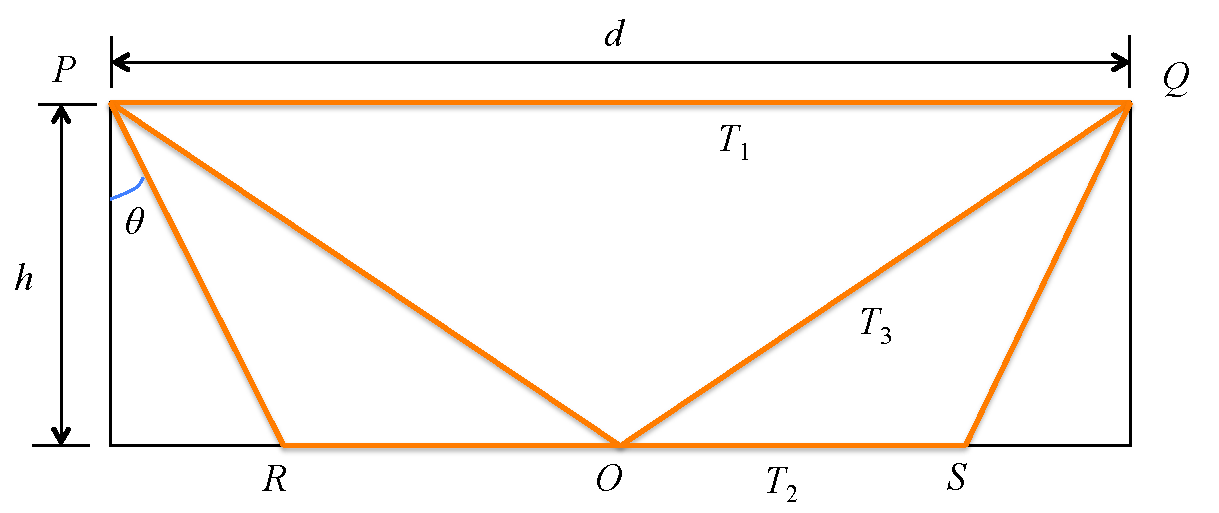
\includegraphics{./images/ch5/eWave.pdf}}
\end{center}

{\bf 提示:}(1)
$$T_1=\df d{c_1}$$
$$T_2=\df{2h}{c_1}\sec\theta-\df{2h}{c_2}\tan\theta+\df d{c_2}$$
$$T_3=\df2{c_1}\sqrt{h^2+\left(\df d2\right)^2}$$


(2)
$$\df{\d T_2}{\d\theta}=\df{2h(c_2\sin\theta-c_1)}{c_1c_2\cos^2\theta}$$
唯一驻点$\sin\theta=\df{c_1}{c_2}$,此时
$$T_2=\df{2h}{c_1c_2}\sqrt{c_2^2-c_1^2}+\df d{c_2}$$

(3)
$$c_1=\df{d}{T_1}\approx3.846km/s$$
$$h=\sqrt{\left(\df{c_1}2T_3\right)^2-\left(\df d2\right)^2}\approx0.4213km$$
又
$$(T_2c_2-d)^2=\df{4h^2}{c_1^2}(c_2^2-c_1^2)$$
解得$c_2=4.1024$或$7.6619$。

{\bf 例:}高度$h$的水桶,顶端不断注水使桶内总是保持水满的状态。在桶的侧面开个小孔,使水喷出。
若小孔距地面高度为$y$,则水喷出的速度为$8\sqrt{h-y}$。问小孔放在多高的位置,能使水喷出的距离
最远。

{\bf 提示:}$y\in(0,h)$,水落地的时间为$\sqrt{2y/g}$,从而喷出的距离
$$s(y)=\df{8\sqrt{2}}{\sqrt g}\sqrt{y(h-y)},$$
$s'(y)=\df{8\sqrt{2}}{\sqrt g}\df{h-2y}{2\sqrt{y(h-y)}}$,唯一驻点$y=\df h2$。
显然其为最大值点,$s_{\max}=\df{4\sqrt 2}{\sqrt{g}}h$

{\bf 例:}同一维度上两座建筑物,间隔$l=50$(m),高度分别为$h_1=60$(m)和
$h_2=30$(m),在两个建筑物间修一座太阳能
站,如何选址方为最优?

{\bf 提示:}使
$$\theta=\pi-\arctan\df{h_1}{x}-\arctan\df{h_2}{l-x}$$
最大。
$$\theta'_x=\df{h_1}{h_1^2+x^2}-\df{h_2}{h_2^2+(l-x)^2}$$
$$\left(x-\df{lh_1}{h_1-h_2}\right)^2-h_1h_2\left(\df{l^2}
{(h_1-h_2)^2}+1\right)=0$$

{\bf 提示:}能保证最长的日照时间应为最优。结果为距较高的一侧约29.5m。

{\bf 例:}如图,从原点处发出的炮弹,求
\begin{enumerate}[(1)]
  \setlength{\itemindent}{1cm}
  \item 炮弹轨迹的参数方程
  \item 何时炮弹的射程最远
  \item 如果坡面是向上的呢?
\end{enumerate}
\begin{center}
	\resizebox{!}{5cm}{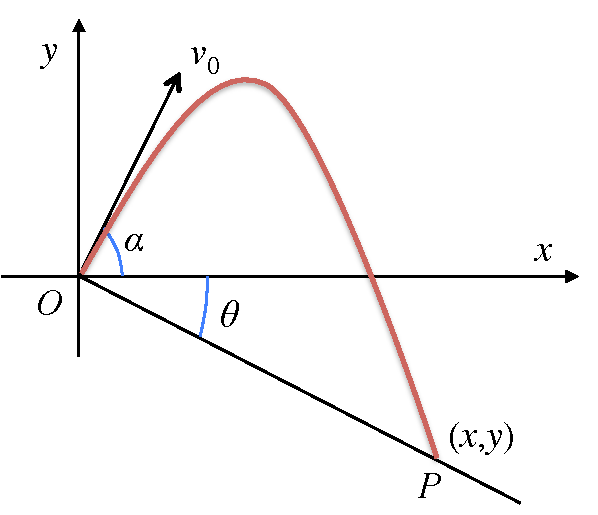
\includegraphics{./images/ch5/bFly.pdf}}
\end{center}

{\bf 提示:}(1)以时间$t$为参数,则
$$x=(v_0\cos\alpha)t,\quad y=(v_0\sin\alpha)t-\df12gt^2$$
消去$t$,可得$y=x\tan\alpha-\df{gx^2}{2v_0^2\cos^2\alpha}$。落点处满足
$y=-x\tan\theta$,联立解得
$$x=\df{2v_0^2\cos^2\alpha}g(\tan\alpha+\tan\theta),$$
从而炮弹的飞行时间
$$T=\df x{v_0\cos\alpha}=\df{2v_0\cos\alpha}g(\tan\alpha+\tan\theta),$$
从而参数$t\in[0,T]$。

(2)射程
$$R(\alpha)=x\sec\theta=\df{2v_0^2}{g\cos^2\theta}\cos\alpha\sin(\alpha+\theta),$$
$$R'(\alpha)=\df{2v_0^2}{g\cos^2\theta}\cos(2\alpha+\theta),$$
驻点$\alpha=\df12\left(\df{\pi}2-\theta\right)$

(3)使用$-\theta$替换$\theta$,最大值点$\alpha=\df12\left(\df{\pi}2+\theta\right)$

\begin{shaded}
% {\bf 【其他有趣的应用】}

{\bf 关于$\left(1+\df1n\right)^n\to e(n\to\infty)$的另一个证明}

{\bf 例:}$f_u(x)=x^ue^{-x}(x\geq0)$,对于确定的$u>0$,证明
\begin{enumerate}[(1)]
  \setlength{\itemindent}{1cm}
  \item $f_u(x)$在$x=u$处达到最大值;
  \item 由$f_u(u)>f_u(u+1)$和$f_{u+1}(u+1)>f_u(u)$推出
  $$\left(\df{u+1}u\right)^u<e<\left(\df{u+1}u\right)^{u+1}$$
  \item 由$\df{u}{u+1}<\left(\df{u+1}u\right)^u<e$推出
  $\lim\limits_{u\to+\infty}\left(1+\df1u\right)^u=e$
\end{enumerate}

\end{shaded}

\section{微分中值定理}

\subsection{Rolle定理}

{\bf 定理5.2.1:}若函数$f(x)$满足:
\begin{enumerate}[(1)]
  \setlength{\itemindent}{1cm}
  \item 在区间$[a,b]$上连续
  \item 在区间$(a,b)$内可导
  \item $f(a)=f(b)$
\end{enumerate}
则:存在$\xi\in(a,b)$,使得$f\,'(\xi)=0$。

{\bf 注:}{\b 三个条件缺一不可!!}\ps{为什么?每种情况给出相应的反例!}

{\bf 例:}证明:对函数$f(x)=(x-1)(x-2)(x-3)$,至少存在一点
$\xi\in(1,3)$,使得$f\,''(\xi)=0$。

{\bf 例}(Darboux定理)设$f(x)$在$[a,b]$上可导,且$f\,'_+(a)f\,'_-(b)<0$,
则存在$\xi\in(a,b)$,使得$f\,'(\xi)=0$。

[提示]:不妨设$f'_+(a)>0$,且$f(a)>f(b)$,则可以证明必存在$c\in(a,b)$,
使得$f(c)=f(a)$,然后使用Rolle定理。

{\bf 例:}设$f(x)$在$[a,b]$上满足Rolle定理条件,
且$f\,'_+(a)f\,'_-(b)>0$,则$f\,'(0)=0$在$(a,b)$内至少有两个根。

[提示]:利用极限的保号性,说明在$a,b$附近各有一点,两点函数值反号,然后利用
介值定理和Rolle定理。

{\bf 例:}设$\df{a_0}{n+1}+\df{a_1}{n}+\ldots+a_n=0$,证明:方程
$$a_0x^n+a_1x^{n-1}+\ldots+a_n=0$$
在区间$(0,1)$内至少有一个根。

[提示]:令
$$F(x)=\df{a_0}{n+1}x^{n+1}+\df{a_1}{n}x^n+\ldots+a_nx$$

{\bf 推论}(Rolle定理的高阶推广)
设$f(x)$在$[x_0,x_n]$上有$n-1$阶连续导数,在$(x_0,x_n)$内
$n$阶可导,且
$$f(x_0)=f(x_1)=\ldots=f(x_n),\quad(x_0<x_1<\ldots<x_n),$$
则存在$\xi\in(x_0,x_n)$,使得$f^{(n)}(\xi)=0$。

[提示]:反复使用Rolle定理。

{\bf 例:}设$f(x)\in C[a,b]$,在$(a,b)$内可导,且$f(a)=f(b)=0$,证明:存在
$\xi\in(a,b)$,使得:
$$f'(\xi)+f(\xi)=0.$$

[提示]:$F(x)=f(x)e^x$

{\bf 注:}{\b 辅助函数的构造可以从不定积分中获得一些启发
\begin{itemize}
  \setlength{\itemindent}{1cm}
  \item $f(\xi)+\lambda f'(\xi)=0$:令$F(x)=e^{\lambda x}f(x)$
  \item $f'(\xi)+f(\xi)g'(\xi)=0$: 令$F(x)=e^{\lambda g(x)}f(x)$
  \item $nf(\xi)+xf'(\xi)=0$: 令$F(x)=x^nf(x)$ 
  \item $f'(\xi)g(\xi)+f(\xi)g'(\xi)=0$:令$F(x)=f(x)g(x)$
  \item $f'(x)g(x)-f(x)g'(x)=0$: 令$F(x)=\df{f(x)}{g(x)}$
\end{itemize}
}


\subsection{Lagrange中值定理}

{\bf 定理5.2.2:}若函数$f(x)$满足: 
\begin{enumerate}[(1)]
  \setlength{\itemindent}{1cm}
  \item 在区间$[a,b]$上连续 
  \item 在区间$(a,b)$内可导 
\end{enumerate}
则:{\b 存在$\xi\in(a,b)$,使得 
$$f\,'(\xi)=\df{f(b)-f(a)}{b-a}.$$}

[证明概要]:结论即为\ps{\b 从结论出发构造辅助函数是证明中值问题的常用思路}
$$f'(\xi)(b-a)-[f(b)-f(a)]=0,$$
考虑
$$F'(x)=f'(x)(b-a)-[f(b)-f(a)],$$
从而
$$F(x)=f(x)(b-a)-[f(b)-f(a)]+C,$$
不妨令$C=0$,可以验证$F(b)=F(a)$,在利用Rolle定理即可。

{\bf 注:}Lagrange中值定理的几种常见形式
$${\b f(b)-f(a)=f'(\xi)(b-a)}$$
$${\b f(x+\Delta x)=f(x)+f'(x+\theta\Delta x)\Delta x,
\quad (\theta\in(0,1))}$$

{\bf 推论(教材-例1)}
\begin{enumerate}[(1)]
  \setlength{\itemindent}{1cm}
  \item 导数恒为零的函数取值恒为常数。
  \item 导数恒大于零的函数严格单调递增。
\end{enumerate}

{\bf 教材-例3:}证明方程$x^5+x-1=0$只有唯一实根。

{\bf 例:}证明:$\df{\ln x-\ln x_1}{x-x_1}<\df 1{x_1},\quad (0<x_1<x)$

{\bf 教材-例2:}证明不等式:$\df{x}{1+x}<\ln(1+x)<x,\;x>0$

{\bf 注:}在证明Eular常数
$$\gamma=\limn\left(1+\df12+\ldots+\df1n-\ln n\right)$$
时,用到了这个不等式。

{\bf 教材-例4:}设$f(x)\in C[a,b]$,且$f(x)$在$(a,b)$内二阶可导,
连接函数曲线两端点的直线在$(a,b)$内至少与曲线存在一个交点,
则存在$\xi\in(a,b)$,使得$f\,''(\xi)=0$。

{\bf 思考:}{\b 若光滑曲线的端点连线与函数曲线存在多个交点,能够得到什么结论?}

利用与Lagrange中值定理相似的思想,可以证明:

{\bf 例:}设$f(x)$在$[a,b]$上二阶可导,$f(a)=f(b)=0$,证明:对任意
$c\in(a,b)$,存在$\xi\in(a,b)$,使得
$$f(c)=\df{f\,''(\xi)}{2}(c-a)(c-b)$$
[提示]:设
$$F''(x)=f''(x)-\df{2f(c)}{(c-a)(c-b)},$$
则可得
$$F(x)=f(x)-\df{f(c)}{(c-a)(c-b)}x^2+C_1x+C_2,$$
其中$C_1,C_2$为常数。不妨令$C_1=C_2=0$,以下可以验证:
$$\df{F(c)-F(a)}{c-a}=\df{F(b)-F(c)}{b-c}
=-\df{f(c)}{(c-a)(c-b)}(a+b),$$
由Lagrange中值定理,存在$\xi_1\in(a,c),\xi_2\in(c,b)$,使得
$$F'(\xi_1)=F'(\xi_2)=-\df{f(c)}{(c-a)(c-b)}(a+b),$$
进而再由Rolle定理,存在$\xi\in(\xi_1,\xi_2)$,使得$F''(\xi)=0$,即证。

{\bf 注:}直接令辅助函数
$$F(x)=f(x)-\df{(x-a)(x-b)}{(c-a)(c-b)}f(c)$$
亦可,这个辅助函数的右半部分事实上是过$(a,0),(b,0),(c,f(c))$
三点的Lagrange插值多项式!

\begin{shaded}
{\bf 过$n$个点$(x_i,f(x_i))(i=1,2,\ldots,n)$的Lagrange插值多项式}
$$L_n(x)=\sum\limits_{i=1}^n\prod_{j=1,j\ne i}^{n}
\df{x-x_j}{x_i-x_j}f(x_i)$$

{\bf 例:}过点$(0,0),(1,2),(2,-1),(3,-2)$的Lagrange插值多项式为
$$L(x)=\df{x^3}6-8x^2+\df{41}6x$$

\begin{center}
	\resizebox{!}{5cm}{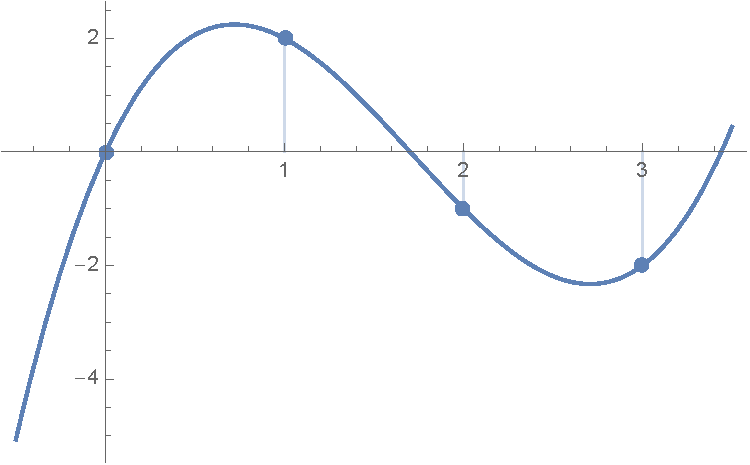
\includegraphics{./images/ch5/L4x.pdf}}
\end{center}

%% code of Mathematica 
% f[x_] := 7/6*x^3 - 6 x^2 + 41/6*x;
% CCurve = Plot[f[x], {x, -0.5, 3.5}];
% DCurve = ListPlot[Table[{n, f[n]}, {n, 0, 3}], Filling -> Axis];
% Show[CCurve, DCurve]

\end{shaded}

\subsection{Cauchy中值定理}

{\bf 定理5.2.3:}若函数$f(x),\varphi(x)$满足: 
\begin{enumerate}[(1)]
  \setlength{\itemindent}{1cm}
  \item 在$[a,b]$上连续 
  \item 在$(a,b)$内可导,且$\varphi'(x)\ne 0$ 
\end{enumerate}
则:存在$\xi\in(a,b)$, 使得
$$\df{f(b)-f(a)}{\varphi(b)-\varphi(a)}=\df{f'(\xi)}{\varphi'(\xi)}$$

[证明概要]:结论即为
$$[f(b)-f(a)]\varphi'(\xi)-[\varphi(b)-\varphi(a)]f'(\xi)=0,$$
因此考虑
$$F'(x)=[f(b)-f(a)]\varphi'(x)-[\varphi(b)-\varphi(a)]f'(x),$$
从而
$$F(x)=[f(b)-f(a)]\varphi(x)-[\varphi(b)-\varphi(a)]f(x)+C.$$
不妨令$C=0$,可以验证$F(b)=F(a)$,利用Rolle定理即可。

{\bf 注:}Cauchy中值定理可视为{\it 参数化}的Lagrange中值定理,即:
由$\varphi'(x)\ne 0$可知,$\varphi(x)$为单调(可逆)函数,从而设
$A=\varphi(a),B=\varphi(b)$,故由Lagrange中值定理,存在$\xi\in(a,b)$,
也即$C=\varphi(\xi)$介于$A,B$之间,使得
$$\df{f(b)-f(a)}{\varphi(b)-\varphi(a)}
=\df{f(\varphi^{-1}(B))-f(\varphi^{-1}(A))}{B-A}
=[f(\varphi^{-1}(x))]'_{x=\xi}=\df{f'(\xi)}{\varphi'(\xi)}.$$

{\bf 例:}设$0<a<b$,$f(x)$在$[a,b]$上连续,在$(a,b)$内可导,证明:
\begin{enumerate}[(1)]
  \setlength{\itemindent}{1cm}
  \item 存在$\xi\in(a,b)$,使得:
	$$f(b)-f(a)=\ln\df ba\cdot \xi f\,'(\xi)$$
  \item 存在$\eta\in(a,b)$,使得:
    $$2\eta[f(b)-f(a)]=(b^2-a^2)f\,'(\eta)$$
  \item 存在$x_1,x_2,x_3\in(a,b)$,使得
	$$f\,'(x_1)=(b+a)\df{f\,'(x_2)}{2x_2}=(a^2+ab+b^2)
	\df{f\,'(x_3)}{3x_3^2}$$ 
  \item 若$f\,'(x)\ne 0$,则存在$\xi,\eta\in(a,b)$,使得
	$$\df{f'(\xi)}{f'(\eta)}=\df{e^b-e^a}{b-a}e^{-\eta}$$
  \item 存在$c\in(a,b)$,使得
	$$\df{1}{a-b}\left|\begin{array}{cc}
	a & b\\ f(a) & f(b)
	\end{array}\right|=f(c)-cf'(c).$$
\end{enumerate}

{\bf 注:}通过对结论适当地变形整理,以上问题都可以使用
Rolle定理证明。

\subsection{L'Hospital法则}

{\bf 不定式(型)极限}
$$\bm{\df{0}{0}}, \quad \bm{\df{\infty}{\infty}}, \quad
\bm{1^{\infty}}, \quad \bm{0\cdot\infty}, \quad
\bm{\infty-\infty}, \quad \bm{\infty^0}, \bm{\quad 0^0}$$

{\bf 注:}以上$0,1,\infty$均表示一种趋势,而不是具体的值!

{\bf 举例:}
\begin{enumerate}[(1)]
  \setlength{\itemindent}{1cm}
  \item $\limx{0}\df{x-\sin x}{x}$ 
  \item $\limx{+\infty}\df{\ln x}{x}$ 
  \item $\limx{1}(1-x^2)\tan\df{\pi}2x$ 
  \item $\limx{0}(x^2+2^x)^{1/x}$
\end{enumerate}

{\bf 定理5.2.4}($0/0$型不定式极限)
设函数$f(x),g(x)$满足: 
\begin{enumerate}[(1)]
  \setlength{\itemindent}{1cm}
  \item $\limx{a^+}f(x)=\limx{a^+}g(x)=0$ 
  \item $f(x),g(x)$在$(a,a+\delta)$内可导,且$g'(x)\ne 0$ 
  \item $\limx{a^+}\df{f'(x)}{g'(x)}$存在 (或等于$\infty$) 
\end{enumerate}
则
$$\limx{a^+}\df{f(x)}{g(x)}=\limx{a^+}\df{f'(x)}{g'(x)}$$

[证明概要]:不妨设$f(a)=g(a)=0$,则由Cauchy中值定理,存在$\xi\in(a,x)$,
$$\df{f(x)}{g(x)}=\df{f(x)-f(a)}{g(x)-g(a)}
=\df{f'(\xi)}{g'(\xi)},$$
注意到{\b$x\to a^+\Leftrightarrow\xi\to a^+$},故
$$\limx{a^+}\df{f(x)}{g(x)}=\limx{a^+}\df{f'(\xi)}{g'(\xi)}
=\lim\limits_{\xi\to a^+}\df{f'(\xi)}{g'(\xi)}
=\limx{a^+}\df{f'(x)}{g'(x)},$$
即证。

{\bf 注:}以上结论可以直接推广到$\infty/\infty$不定式的情形,但需要注意的是
{\b 由$\limx{\Delta}\df{f'(x)}{g'(x)}=A$可以推出
$\limx{\Delta}\df{f(x)}{g(x)}=A$,但反之不然。}反例如下:
$\limx{+\infty}\df{x+\sin x}x=1$,
但$\limx{+\infty}(1+\cos x)$不存在!

参考L'Hospital法则的证明原理,可以证明下面的两个结论:

{\bf 例:}设$\limx{+\infty}f(x)$和$\limx{+\infty}f\,'(x)$均存在,证明:
$$\limx{+\infty}f\,'(x)=0.$$

证:由Lagrange中值定理,对任意$x\in\mathbb{R}$,存在$\xi\in[x,x+1]$,满足
$$f(x+1)-f(x)=f'(\xi),$$
注意到{\b$x\to+\infty\Leftrightarrow\xi\to+\infty$},
$\limx{+\infty}f(x+1)=\limx{+\infty}f(x)$,故
$$0=\limx{+\infty}[f(x+1)-f(x)]=\limx{+\infty}f'(\xi)
=\lim\limits_{\xi\to+\infty}f'(\xi)=\limx{+\infty}f'(x)$$
即证。

{\bf 例:}设$f(x)$在$U(x_0)$内连续,在$U^0(x_0)$内可导,
且$\limx{x_0}f\,'(x)=l$,则$$f\,'(x_0)=l.$$

证:由Lagrange中值定理,对任意$\Delta x\in\mathbb{R}$,存在
$\xi\in[x_0,x_0+\Delta x]$,使得
$$\df{f(x_0+\Delta x)-f(x_0)}{\Delta x}=f'(\xi),$$
注意到$\Delta x\to 0\Leftrightarrow\xi\to0$,故
$$f'(x_0)=\lim\limits_{\Delta x\to 0}\df{f(x_0+\Delta x)-f(x_0)}{x_0}
=\lim\limits_{\Delta x\to 0}f'(\xi)=\lim\limits_{\xi\to 0}f'(\xi)=l,$$
即证。

{\bf 教材-例5-13}
\begin{enumerate}[(1)]
  \setlength{\itemindent}{1cm}
  \item $\limx{0}\df{x-\sin x}{x^3}$ 
  \item $\limx{0}\df{e^x-e^{-x}-2x}{\tan^3x}$ 
  \item $\limx{0}\df{(1+x)^{1/x}-e}{x}$ 
  \item $\limx{+\infty}\df{x^n}{e^{\lambda
  x}}(n\in\mathbb{N},\lambda>0)$ 
  \item $\limx{+\infty}\df{\ln x}{x^\alpha}(\alpha>0)$ 
  \item $\limx{\infty}\df{x+\sin x}{x+\cos x}$
  \item $\limx{1}(1-x^2)\tan\df{\pi}{2}x$ 
  \item $\limx{0}\left(\df 1{x^2}-\df 1{x\tan x}\right)$ 
  \item $\limx{0^+}x^x$
  \item $\limx{0}(x^2+2^x)^{1/x}$ 
  \item $\limx{0}\left(\cot x-\df 1x\right)$ 
  \item $\limn\sqrt[n]n$
\end{enumerate}

不定式极限通常可以进行如下的相互转换

\begin{center}
	\resizebox{!}{4cm}{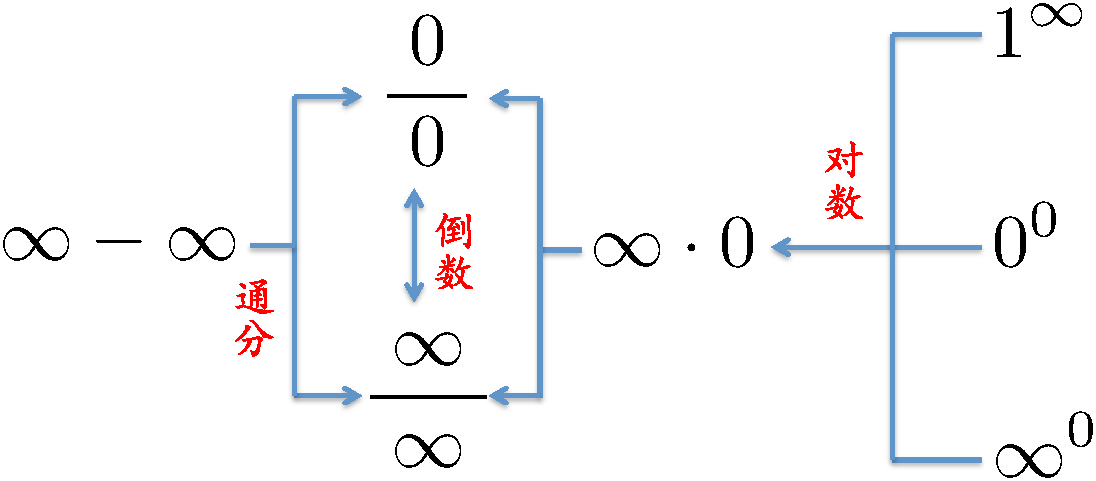
\includegraphics{./images/ch5/lim00.pdf}}
\end{center}

{\b{\bf 习题5.2-15:}设$f(x)$在$x_0$附近存在二阶连续导函数,则
$$\lim\limits_{h\to 0}\df{f(x_0+h)+f(x_0-h)-2f(x_0)}{h^2}=f\,''(x_0).$$
若条件减弱为“$f(x)$在$x=x_0$处二阶可导”,结论是否仍然成立?\ps{难点!}

[提示]:成立,但是如下推导是不对的
\begin{align}
	\lim\limits_{h\to 0}&\df{f(x_0+h)+f(x_0-h)-2f(x_0)}{h^2}
	=\lim\limits_{h\to 0}\df{f'(x_0+h)-f'(x_0-h)}{2h}\notag\\
	&=\lim\limits_{h\to 0}\df{f''(x_0+h)+f''(x_0-h)}{2}
	=f''(0)\notag
\end{align}
其中的错误在于,条件中只有$f(x)$在$x=x_0$处二阶可导,而不是$f(x)$的二阶导数
在$x_0$附近连续,因此最后的两个等号都是不成立的!

事实上,正确的推导应该是
\begin{align}
	\lim\limits_{h\to 0}&\df{f(x_0+h)+f(x_0-h)-2f(x_0)}{h^2}
	=\lim\limits_{h\to 0}\df{f'(x_0+h)-f'(x_0-h)}{2h}\notag\\
	&=\df12\lim\limits_{h\to 0}\df{f'(x_0+h)-f'(x_0)}{h}
	+\df12\lim\limits_{h\to 0}\df{f'(x_0-h)-f'(x_0)}{-h}
	=f''(0)\notag
\end{align}
其中最后一个等号只用到了二阶导数的定义。}

{\bf 例:}
设$f(0)=1$,且
$$\limx{0}\df{\ln(1-x)+f(x)\sin x}{e^{x^2}-1}=0,$$
证明:$f(x)$在$x=0$处可导,求$f\,'(0)$。

\section{Taylor公式与函数的多项式逼近}

\subsection{Taylor多项式}

{\bf 定义:}$P_n(x)$称为{\it $f(x)$在点$x_0$处的$n$阶Taylor多项式}
\ps{注意Taylor多项式、Taylor公式和Taylor级数的区别},若
\begin{itemize}
  \setlength{\itemindent}{1cm}
  \item $P_n(x)$是$n$次多项式,形如:$\sum\limits_{k=0}^na_k(x-x_0)^k$
  \item $y=P_n(x)$在$x_0$处与$y=f(x)$处至少{\it $n$阶相切},即
  对任意$k=0,1,2,\ldots,n$,有
  $$P^{(k)}_n(x_0)=f^{(k)}(x_0)$$
%   \begin{enumerate}[(1)]
%     \item $P_n(x_0)=f(x_0)$
%     \item $P'_n(x_0)=f'(x_0)$
%     \item $P''_n(x_0)=f''(x_0)$
%     \item \ldots
%     \item $P^{(n)}_n(x_0)=f^{(n)}(x_0)$
%   \end{enumerate} 
\end{itemize}
若$x_0=0$,称为{\it $f(x)$的$n$阶Maclaurin多项式}

根据以上定义,可推得\ps{\b 给定$f(x)$、$x_0$和$n$,$P_n(x)$唯一确定}
$${\b P_n(x)=\sum\limits_{k=0}^n\df{f^{\,(k)}(x_0)}{k!}(x-x_0)^k}$$

{\bf 教材-例1-2:}求Maclaurin多项式
\begin{enumerate}[(1)]
  \setlength{\itemindent}{1cm}
  \item $f(x)=e^x$ 
  $${P_n(x)=1+x+\df{x^2}{2!}+\ldots+\df{x^n}{n!}}$$ 
  \item $f(x)=\cos x$ 
  $${P_{2m}(x)=1-\df{x^2}{2!}+\df{x^4}{4!}-\ldots+(-1)^m\cdot\df{x^{2m}}{(2m)!}}$$
\end{enumerate}

\subsection{误差估计}

{\bf 定理5.3.1:}
设函数$f(x)$在$x_0$处$n$阶可导,$P(x)$是$f(x)$在点$x_0$处
的$n$阶Taylor多项式,则当$x\to x_0$时
$${|f(x)-P_n(x)|=\circ[(x-x_0)^n]}$$

{\bf 注:}该定理说明多项式逼近是比线性逼近更精确的逼近,也就是
用所谓的“以曲代曲”推广了“以直代曲”

\begin{itemize}
  \setlength{\itemindent}{1cm}
  \item {\it 余项:}$R_n(x)=|f(x)-P_n(x)|$ 
  \item {\it 带Peano余项的$n$阶Taylor公式:}
  $${\b f(x)=P_n(x)+\circ[(x-x_0)^n]}$$
\end{itemize}

{\bf 注:}{\b 阶数是多少,关键看余项!}例如$\sin x$的7阶和8阶Maclaurin公式分别为
$$\sin x=x-\df{x^3}{3!}+\df{x^5}{5!}-\df{x^7}{7!}+{\b\circ(x^7)},$$
$$\sin x=x-\df{x^3}{3!}+\df{x^5}{5!}-\df{x^7}{7!}+{\b\circ(x^8)}.$$

{\bf 定理5.3.2}({\it Taylor中值定理})
设$f(x)$在$x_0$的某邻域内$n+1$阶可导,对该领域内任一点$x$,存在介于
$x_0$和$x$之间的一点$\xi$,满足
$${f(x)=P_n(x)+\df{f^{(n+1)}(\xi)}{\,(n+1)!}(x-x_0)^{n+1}}$$
上式称为{\it 带Lagrange余项的$n$阶Taylor公式}\ps{从这个意义上说,Taylor公式
是对Lagrange中值定理的推广}
$${\b f(x_0+h)=P_n(x_0+h)+\df{f^{\,(n+1)}(x_0+\theta
h)}{(n+1)!}h^{n+1},(0<\theta<1)}$$

证:\ps{这个证明比教材上的方法更为直观!}
先考虑$x>x_0$的情况,其余情况可以类似地证明。注意到$P^{(n+1)}(x)=0$,
$f^{(k)}(x_0)=P^{(k)}_n(x_0),k=0,1,2,\ldots,n$,
反复利用Cauchy中值定理,存在$x_0<\xi<\xi_n<\xi_{n-1}
<\ldots<\xi_2<\xi_1<x$,使得
\begin{align}
	\df{f(x)-P_n(x)}{(x-x_0)^{n+1}}
	&=\df{f'(\xi_1)-P'_n(\xi_2)}{(n+1)(\xi_1-x_0)^{n}}
	=\df{f''(\xi_2)-P''_n(\xi_2)}{(n+1)n(\xi_2-x_0)^{n-1}}\notag\\
	&=\ldots=\df{f^{(n)}(\xi_n)-P^{(n)}_n(\xi_n)}{(n+1)!(\xi_n-x_0)}
	=\df{f^{(n+1)}(\xi)}{(n+1)!}\notag
\end{align}
即证。

{\bf 推论:}若存在常数$C>0$,使当$x\in(a,b)$时,恒有
$$|f^{\,(n+1)}(x)|\leq C,\;n=0,1,2,\ldots$$
则
$$\limn [f(x)-P_n(x)]=0.$$
也即:Taylor多项式的次数越高,逼近精度越高。

{\b
{\bf 例}(常用的Maclaurin公式)
\begin{enumerate}[(1)]
  \setlength{\itemindent}{1cm}
  \item {$e^x =\sum\limits_{k=0}^n\df{x^k}{k!}
  +\df{e^{\theta x}}{(n+1)!}x^{n+1}\;
  (0<\theta<1,x\in\mathbb{R})$}
  \item {$\sin x
  =\sum\limits_{k=1}^m(-1)^{k-1}\df{x^{2k-1}}{(2k-1)!} 
  +(-1)^m\df{\cos\theta x}{(2m+1)!}x^{2m+1}\;
  (0<\theta<1,x\in\mathbb{R})$}
  \item {$\cos x= \sum\limits_{k=0}^m(-1)^{k}\df{x^{2k}}{(2k)!}
  +(-1)^{m+1}\df{\sin\theta
  x}{(2m+2)!}x^{2m+2}\; (0<\theta<1,x\in\mathbb{R})$}
  \item
  {$\ln(1+x) =\sum\limits_{k=1}^n(-1)^{k-1}\df{x^k}{k}
  +\df{(-1)^nx^{n+1}}{(n+1)(1+\theta
  x)^{n+1}}\; (0<\theta<1,x>-1)$} 
  \item
  {$(1+x)^\alpha =\sum\limits_{k=0}^n
  \df{\alpha(\alpha-1)\ldots(\alpha-k+1)}{k!}x^k
	 +\df{\alpha(\alpha-1)\ldots(\alpha-n)}{(n+1)!}\df{x^{n+1}}{(1+\theta
	x)^{n+1-\alpha}}\quad (0<\theta<1,x\ne -1)$}
\end{enumerate}
}

\subsection{函数的Taylor展开}

{\bf 问题:}{ 给定函数$f(x)$,求其在$x_0$的$n$阶Taylor公式} 
\begin{enumerate}[(1)]
  \setlength{\itemindent}{1cm}
  \item {\bf 直接法(公式法)} 
  \begin{itemize}
    \item 逐个计算Taylor系数,给出相应的公式 
  \end{itemize}
  \item {\bf 间接法} \ps{能够使用间接法求展开的根本原因是Taylor展开具有唯一性!}
  \begin{itemize}
    \item 利用已知函数的Maclaurin公式 
    \item 利用级数和多项式的性质
  \end{itemize}
\end{enumerate}

\subsubsection{【多项式函数的展开】}

{\bf 定理}
多项式函数$P_n(x)=\sum\limits_{k=0}^na_kx^k$的$m$阶Maclaurin多项式为其$m$次
{\it 截断多项式:} 
$${P_m(x)=\sum\limits_{k=0}^ma_kx^k}$$

{\bf 教材-习题1:}求$f(x)=x^3+3x^2-2x+4$的各阶Maclaurin多项式和在
$x=1$处的Taylor多项式。

[提示]:{\b$f(x)$自身已经是一个Maclaurin多项式,但若所求展开式是在某个$x_0$处,
则应该使用形如$t=x-x_0$的变化先求对应的Maclaurin公式,再代回即可。}

\subsubsection{【直接法求Taylor展开式】}

{\bf 教材-例3:}求$f(x)=\tan x$的$3$阶带有Peano余项的Maclaurin公式。

\begin{itemize}
  \setlength{\itemindent}{1cm}
  \item 直接法:逐阶求导,然后展开
  \item 待定系数法:利用$\sin x$和$\cos x$的展开式,确定相关的系数
\end{itemize}

\subsubsection{【间接法求Taylor展开式】}

{\bf 规则一:}若在区间$I$内,$f(x)=\sum\limits_{n=0}^{\infty}a_nx^n$,
$g(x)=\sum\limits_{n=0}^{\infty}b_nx^n$,则
\begin{enumerate}[(1)]
  \setlength{\itemindent}{1cm}
  \item $\lambda f(x)+\mu g(x)=\sum\limits_{n=0}^{\infty}(\lambda a_n+\mu
  b_n)x^n$,其中$\lambda,\mu$为常数 
  \item $f\,'(x)=\sum\limits_{n=0}^{\infty}na_{n}x^{n-1}$ 
  \item $\displaystyle\int f(x)dx=\sum\limits_{n=0}^{\infty}
  \df{a_{n}}{n+1}x^{n+1}$
\end{enumerate}

{\bf 教材-例4:}求$f(x)=\df 12\ln\df{1+x}{1-x}$的$n$阶带有Peano余项的Maclaurin公式。

{\b{\bf 教材-例5:}求$f(x)=\df 1{2+x}$在$x=1$处的$7$阶Taylor多项式,并求$f^{(7)}(1)$。

[提示]:
$$f(x)=\df13\cdot\df1{(x-1)/3+1}=\sum\limits_{k=0}^n
\df{(-1)^{k}}{3^{k+1}}(x-1)^{k}+\circ((x-1)^n)$$
$${\b f^{(7)}(1)=7!\cdot a_7=-\df{7!}{3^8}}$$
}

{\bf 例:}设$y=\arctan x$,求$y^{(n)}(0)$\ps{4.2节介绍
求高阶导数的Leibniz公式时曾做过此题}

[提示]
$$y'=\df1{1+x^2}=\sum\limits_{k=0}^{\infty}{(-1)^k}x^{2k},\quad (|x|<1),$$
故(逐项积分)可得
$$\arctan x=\sum\limits_{k=0}^{\infty}\df{(-1)^k}{2k+1}x^{2k+1},
\quad (|x|<1),$$
从而可知
$$y^{(n)}(0)=\left\{\begin{array}{ll}
0,& n=2k,\\ {(-1)^k}(2k)!,& x=2k+1
\end{array}\right.$$

{\bf 规则二:}若在区间$I$上,恒有$f(x)=\sum\limits_{n=1}^{\infty}a_nx^n$,
给定函数$g(x)$,当$g(x)\in I$时,恒有
$$f[g(x)]=\sum\limits_{n=1}^{\infty}a_n[g(x)]^n.$$

{\b{\bf 习题5.3-4:}求带有Peano余项的Maclaurin公式\ps{请特别注意高阶无穷小的简化}
\begin{enumerate}[(1)]
  \setlength{\itemindent}{1cm}
  \item $f(x)=\ln(2+x)=\ln2+\ln\left(1+\df x2\right)
  =\ln2+\sum\limits_{k=1}^n\df{(-1)^{k-1}}{k2^k}x^k+\circ(x^n)$ 
  \item $f(x)=e^{-x^2}=\sum\limits_{k=0}^n\df{(-1)^k}{k!}x^{2k}
  +\circ(x^{2n})$
  \item $f(x)=x\sin x=\sum\limits_{k=0}^{n}\df{(-1)k}{k!}x^{2k+2}
  +\circ(x^{2n+2})$ 
  \item $f(x)=\df{x^2}{1+x}=\sum\limits_{k=0}^n(-1)^kx^{k+2}
  +\circ(x^{n+2})$ 
  \item $f(x)=\df{1}{\sqrt{1-x^2}}=\sum\limits_{k=0}^n\left(
  \begin{array}{c}
  -\frac12\\ k
  \end{array}\right)(-1)^kx^{2k}+\circ(x^{2n})$ 
  \item $f(x)=\cos^2x=\df{1+\cos2x}2=\df12+
  \sum\limits_{k=0}^{n}\df{(-1)^k2^k}{(2k)!}x^{2k}+\circ(x^{2n})$
\end{enumerate}}

\subsection{Taylor公式的应用}

\subsubsection{【近似计算】}

{\bf 教材-例6:}计算$e$的值,误差不超过$10^{-5}$。

\begin{center}
	\resizebox{!}{5.5cm}{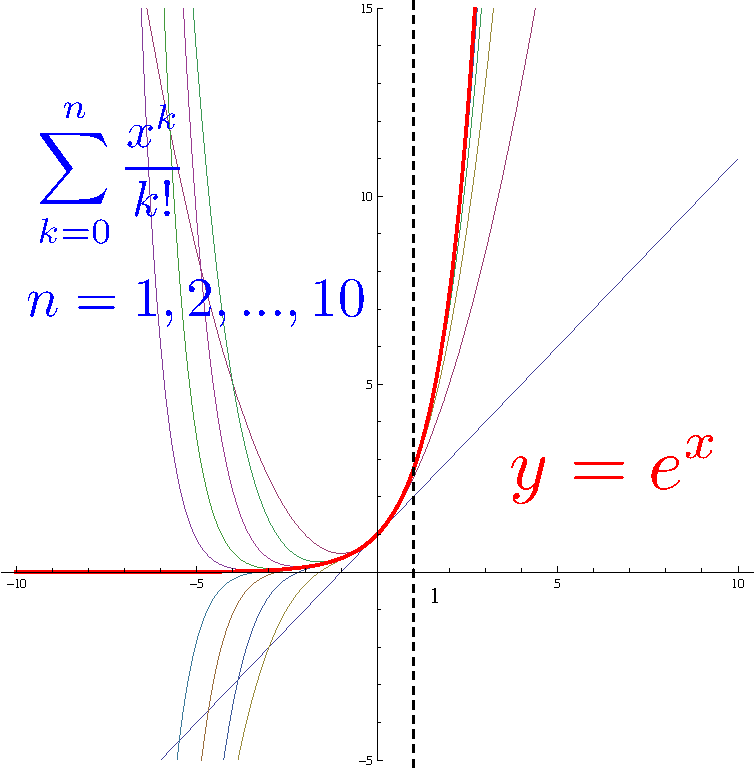
\includegraphics{./images/ch5/exse1.pdf}}\quad
	\resizebox{!}{5.5cm}{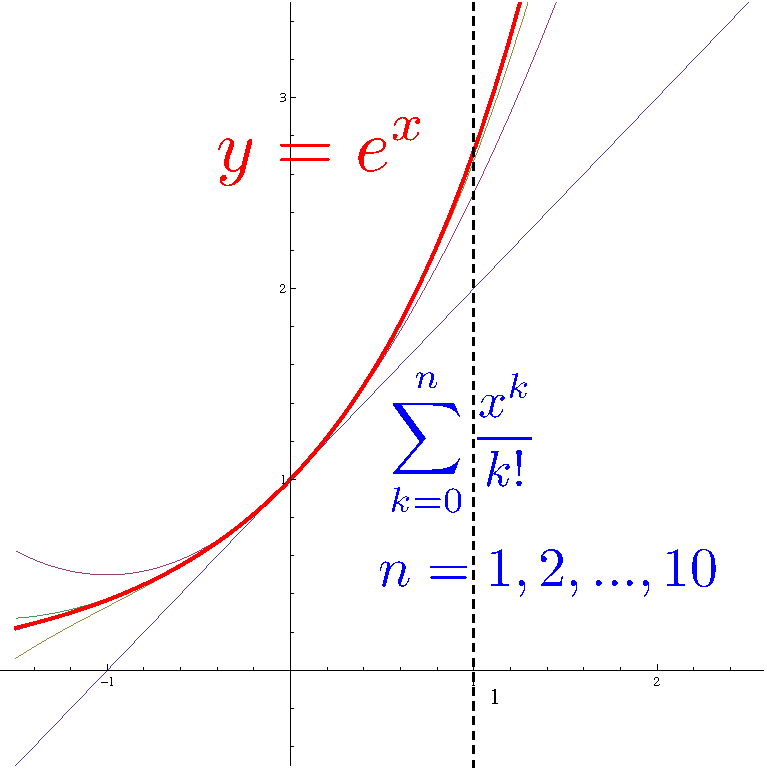
\includegraphics{./images/ch5/exse2.pdf}}
\end{center}

\subsubsection{【计算不定式极限】}

{\bf 教材-例8:}计算以下极限\ps{\b 重点!难点!考点!}
\begin{enumerate}[(1)]
  \setlength{\itemindent}{1cm}
  \item $\limx{0}\df{x-\sin x}{x^3}
  =\limx0\df{x-[x-\frac{x^3}3!+\circ(x^3)]}{x^3}=\df16$
  \item $\limx{0}\df{\cos x-e^{-x^2/2}}{x^4}
  =\limx0\df{1-\frac{x^2}2+\frac{x^4}{4!}-[1-\frac{x^2}2+
  \frac{x^4}8]+\circ(x^4)}{x^4}=-\df1{12}$ 
  \item $\limx{0}\df{\df{x^2}{2}+1-\sqrt{1+x^2}}{x^2\sin x^2}
  =\limx0\df{\frac{x^2}2+1-[1+\frac12{x^2}-\frac18x^4+\circ(x^4)]}{x^4}
  =\df18$ 
  \item $\limx{0}\df{e^x-1-x}{\df{1}{\sqrt{1+x}}-\cos\sqrt x}
  =\limx0\df{\frac{x^2}2+\circ(x^2)}{1-\frac12x+\frac38x^2-[1-\frac{x}2+\frac{x^2}{4!}]+\circ(x^2)}
  =\df32$ 
  \item $\limx{0}\df{\cos(\sin x)-\cos x}{x^4}
  =-2\limx0\df{\sin\frac{\sin x+x}2\sin\frac{\sin x-x}2}{x^4}=\df16$
  \item $\limx{+\infty}\left[x-x^2\ln\left(1+\df 1x\right)\right]
  \xlongequal{u=1/x}\lim\limits_{u\to0}\df{u-\ln(1+u)}{u^2}$
\end{enumerate}

{\bf 注:}不知道该展开到多少阶时,先进行试探性展开

{\bf 例:}设$f(x)$在$x=0$附近二次可导,且
$$\limx{0}\left(1+x+\df{f(x)}{x}\right)^{1/x}=e^3,$$
求:
\begin{enumerate}[(1)]
  \setlength{\itemindent}{1cm}
  \item $f(0),f\,'(0),f\,''(0)$;
  \item $\limx{0}\left(1+\df{f(x)}{x}\right)^{1/x}$.
\end{enumerate}

{\bf 解:}注意到$1/x\to\infty\;(x\to0)$,故已知极限存在,当且仅当
$$\limx0\left(1+x+\df{f(x)}x\right)=1
\quad\Rightarrow\quad f(0)=\limx0f(x)=0.$$
又原式即为
$$\left\{\limx0\left(1+x+\df{f(x)}{x}\right)
^{\frac{x}{x^2+f(x)}}\right\}^{\limx0\frac{x^2+f(x)}{x^2}}=e^3,$$
故必有
$$\limx0\frac{x^2+f(x)}{x^2}=3\quad\Rightarrow\quad
\limx0\df{f(x)}{x^2}=2,$$
进而
$$f'(0)=\limx0\df{f(x)-f(0)}x=\limx0\df{f(x)}{x^2}\limx0x=0.$$
至此,由Taylor公式,可设$f(x)=\df{f''(0)}2x^2+\circ(x^2)$,于是
$$2=\limx0\df{f(x)}{x^2}=\df{f''(0)}2\quad\Rightarrow\quad
f''(0)=4.$$
综上,$f(x)=2x^2+\circ(x^2)$,
\begin{align}
	\limx{0}\left(1+\df{f(x)}{x}\right)^{1/x}
	&=\limx0(1+2x+\circ(x))^{\frac1x}\notag\\
	&=\left\{\limx0(1+2x+\circ(x))^{\frac1{2x+\circ(x)}}\right\}
	^{\limx0{[2+\circ(1)]}}=e^2.\notag	
\end{align}

\subsubsection{【证明不等式】}

{\bf 教材-例9:}证明:$x>0$时,$e^x>1+x+\df{x^2}{2}$

{\bf 教材-例10:}设$f(x)$在$(a,+\infty)$内具有二阶导数,
且$f(x),f\,''(x)$在$(a,+\infty)$
有界,证明:$f\,'(x)$在$(a,+\infty)$有界。

{\bf 例:}证明:若在$(a,b)$内,$f''(x)>0$,则对任意$a<x_1<x_2<b$,恒有
$$f\left(\df{x_1+x_2}{2}\right)<\df{f(x_1)+f(x_2)}{2}.$$

证:记$c=\df{x_1+x_2}2$,则由Taylor公式,存在$\xi_1\in(x_1,c),
\xi_2\in(c,x_2)$,使得
$$f(x_1)=f(c)+f'(c)\df{x_1-x_2}2+f''(\xi_1)
\left(\df{x_1-x_2}2\right)^2$$
$$f(x_2)=f(c)+f'(c)\df{x_2-x_1}2+f''(\xi_2)
\left(\df{x_2-x_1}2\right)^2$$
两式相加,且由$f''(x)>0$,可得
$$f(x_1)+f(x_2)=2f(c)+[f''(\xi_1)+f''(\xi_2)]
\left(\df{x_2-x_1}2\right)^2>2f(c),$$
即证。

{\bf 思考:}以上结论能否进一步推广?
$${f(\lambda x_1+(1-\lambda)x_2)<\lambda
f(x_1)+(1-\lambda)f(x_2),\;0<\lambda<1}$$

{\bf 例:}设在$f(x)$在$[0,a]$上二阶连续可导,
$|f\,''(x)|\leq M$,且$|f(x)|$在$(0,a)$内可取到最大值,证明:
$$|f\,'(0)+f\,'(a)|\leq Ma.$$

{\bf 例:}设$f(x)$在$[0,1]$上二阶连续可导,且$f(0)=f(1)$,
$|f\,''(x)|\leq A$,证明:对任意$x\in(0,1)$,恒有
$$|f\,'(x)|\leq\df A4.$$

证:由Taylor公式,对任意$x\in(0,1)$,存在$\xi_1\in(0,x),
\xi_2\in(x,1)$,使得
$$f(0)=f(x)+f'(x)(-x)+\df{f''(\xi_1)}2x^2,$$
$$f(1)=f(x)+f'(x)(1-x)+\df{f''(\xi_2)}2(1-x)^2,$$
两式相减,且由$f(0)=f(1)$,可得
$$0=f'(x)+\df12\left[f''(\xi_2)(1-x)^2-f''(\xi_1)x^2\right],$$
由$|f''(x)|\leq A$,故
$$|f'(x)|\leq\df A2[(1-x)^2+x^2],$$
注意到当$x\in(0,1)$时,$(1-x)^2+x^2\leq1$,故$|f'(x)|\leq\df A2$,即证。

{\b{\bf 用Taylor公式证明等式或不等式} 
\begin{itemize}
  \item 多使用Lagrange余项
  \item 特殊的点: 区间端点、 极(最)值点、
  区间中点、 距离为常数的点、 已知条件中提到的特殊点
\end{itemize}}

{\bf 例:}设$f(x)\in C^3[-1,1]$,且$f(-1)=0,f(1)=1,f'(0)=0$,
证明:存在$\xi\in(-1,1)$,使得$f'''(\xi)=3$.

[提示]:将$f(-1),f(1)$在$x=0$处展开到三阶带Lagrange余项的Taylor公式,
然后利用介值定理。

{\bf 辅导书P153-例37:}
设$f(x)$在$[a,b]$上二阶连续可导,且$f_+'(a)=f_-'(b)=0$,则至少存在一点
$c\in(a,b)$,使得
$$|f\,''(c)|\geq \df 4{(b-a)^2}|f(b)-f(a)|.$$

[提示]:将$f\left(\df{a+b}2\right)$在$x=a,b$展开,取绝对值放缩后,
利用介值定理。



\section{函数的单调性、凹凸性}

\subsection{可导函数的单调性与极值}

\subsubsection{【单调性】}

{\bf 定理5.4.1:}设$f(x)$在$[a,b]$上连续,$(a,b)$内可导,且$f\,'(x)$恒大(小)于零,
则$f(x)$在$[a,b]$上严格单调递增(减)。

\begin{itemize}
  \setlength{\itemindent}{1cm}
  \item 以上仅仅是判定可导函数严格单调的充分条件,而非充要条件 
  \item 若定理中的“大(小)于”改成“大(小)于等于”,则对应于单调递增情形,且为充要条件
  \item {\b 若定理中的“大(小)于”改成“大(小)于等于”,且导数知道不可能在任何一段
  连续区间内恒等于零,则可推出函数为{\it 严格}单调}
\end{itemize}

{\bf 定理}(可导函数单调的充要条件)设$f(x)$在$[a,b]$上连续,$(a,b)$内可导,
则$f(x)$在$[a,b]$上严格单调递增,当且仅当:
\begin{enumerate}[(1)]
  \setlength{\itemindent}{1cm}
  \item $f\,'(x)\geq 0,\;x\in(a,b)$
  \item 在$(a,b)$的任意子区间上$f\,'(x)$不恒为零
\end{enumerate}

{\bf 注:}{\b 导函数不变号且只有{\it 孤立零点}的函数严格单调!}

{\bf 教材-例1-2:}讨论$y=x-\sin x$的单调性。\ps{用导数来证明单调性显然比
利用函数的性质直接证明要容易得多}

\begin{center}
	\resizebox{!}{5cm}{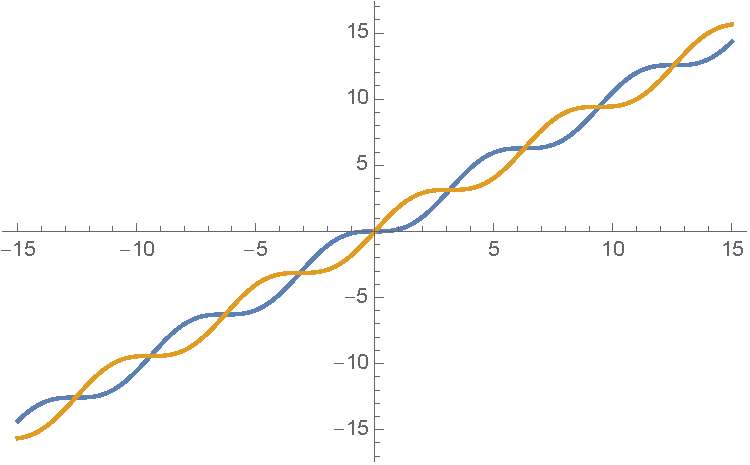
\includegraphics{./images/ch5/xpmSinx.pdf}}
	
	{\it $y=x\pm\sin x$的函数图形}
\end{center}

\subsubsection{【单调性的应用】}

{\bf 推论1:}设$\varphi(x),\psi(x) $均在$[a,b]$上可导,且:
\begin{enumerate}[(1)]
  \setlength{\itemindent}{1cm}
  \item $\varphi'(x)>\psi'(x),\;x\in(a,b)$
  \item $\varphi(a)\geq\psi(a)$
\end{enumerate}
则在$(a,b)$上,恒有$\varphi(x)>\psi(x)$

{\bf 例:}证明:当$x>0$时,恒有
$$x-\df 16x^3<\sin x<x.$$

\begin{center}
	\resizebox{!}{5cm}{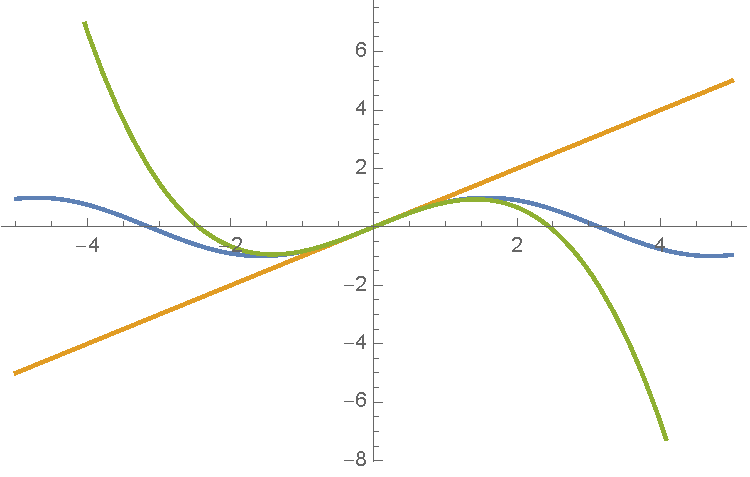
\includegraphics{./images/ch5/xSinxx3.pdf}}
\end{center}

{\b {\bf 推论2:}设$\varphi(x),\psi(x) $均在$[a,b]$上$n$阶可导,且:
\ps{反复多次利用前述推论!}
\begin{enumerate}[(1)]
  \setlength{\itemindent}{1cm}
  \item $\varphi^{(n)}(x)>\psi^{(n)}(x),\;x\in(a,b)$
  \item $\varphi^{(k)}(a)\geq\psi^{(k)}(a),k=0,1,2,\ldots,n-1$
\end{enumerate}
则在$(a,b)$上,恒有$\varphi(x)>\psi(x)$}

{\bf 例:}证明下列不等式
\begin{enumerate}[(1)]
  \setlength{\itemindent}{1cm}
  \item $\ln(1+x)>\df{\arctan x}{1+x},\;(x>0)$
  \item $e^x>1+x+\df
  {x^2}{2!}+\df{x^3}{3!}+\ldots+\df{x^n}{n!},\;(x>0,n\in\mathbb{N})$
\end{enumerate}

\begin{center}
	\resizebox{!}{4cm}{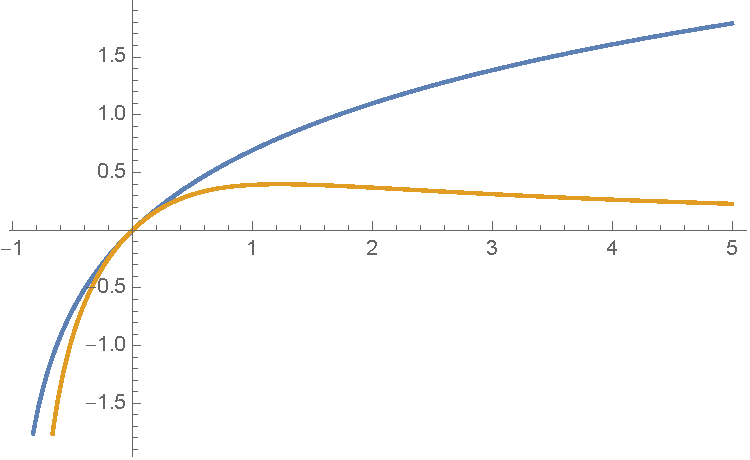
\includegraphics{./images/ch5/lnxArctanx.pdf}}\quad
	\resizebox{!}{4cm}{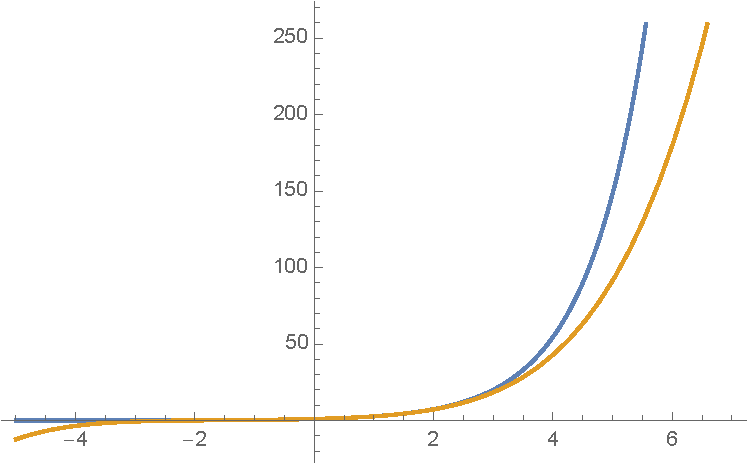
\includegraphics{./images/ch5/exTaylor.pdf}}
\end{center}

\subsubsection{【可导函数的极值】}

{\bf 定理5.4.2}(极值第一充分条件)
设$f(x)$在$x_0$连续,在$x_0$的去心领域内可导,且$f\,'(x)$在$x_0$两侧导数值异号
({\it $f(x)$单调性不同}),则$f(x)$在$x_0$处取极值。\ps{\b 此处不关心$f(x)$在
$x_0$是否可导!}

{\bf 例:}讨论以下函数的极值
\begin{enumerate}[(1)]
  \setlength{\itemindent}{1cm}
  \item $f(x)=2-|x^3-1|$
  \item $f(x)=\left(1+x+\df{x^2}{2!}+\ldots+\df{x^n}{n!}\right)e^{-x}$ 
\end{enumerate}

\begin{center}
	\resizebox{!}{4cm}{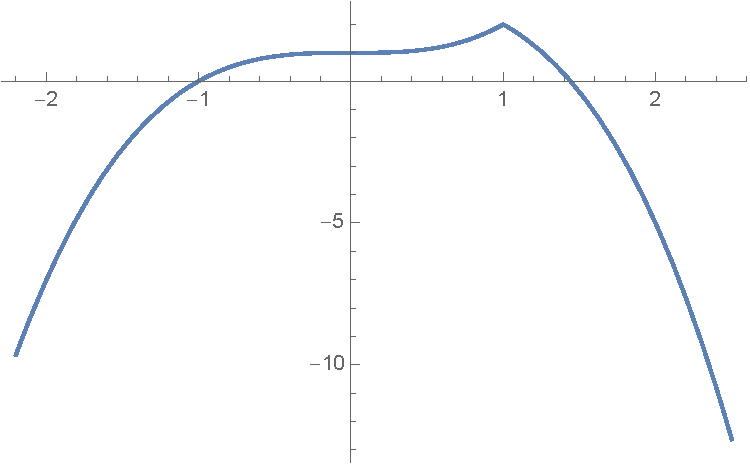
\includegraphics{./images/ch5/2x3.pdf}}\quad
	\resizebox{!}{4cm}{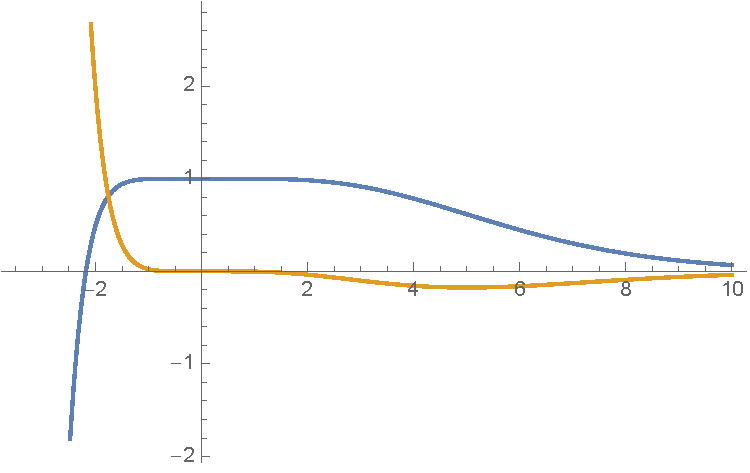
\includegraphics{./images/ch5/1xxe-x.pdf}}
	
	{\it 蓝色和黄色分别为函数和导函数的曲线}
\end{center}

{\bf 定理5.4.3}(极值第二充分条件)\ps{最常用的极值判定方法}
设$f(x)$在$x_0$二阶可导,且$f\,'(x_0)=0$,则
\begin{enumerate}[(1)]
  \setlength{\itemindent}{1cm}
  \item 若$f\,''(x_0)<0$,$f(x)$在$x_0$处取极大值 
  \item 若$f\,''(x_0)>0$,$f(x)$在$x_0$处取极小值
\end{enumerate}

{\bf 例:}讨论以下函数的极值
\begin{enumerate}[(1)]
  \setlength{\itemindent}{1cm}
  \item $f(x)=x^3-6x^2+5$\hfill (教材-例4)
  \item $f(x)=\cos x+\df12\cos 2x$
\end{enumerate}

\begin{center}
	\resizebox{!}{4cm}{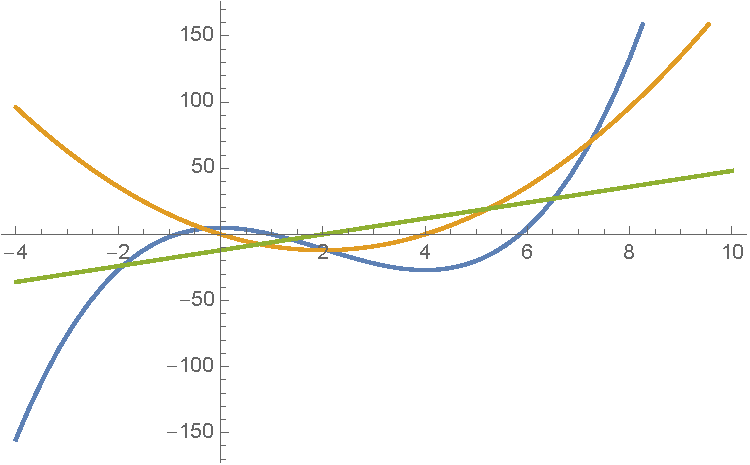
\includegraphics{./images/ch5/x36x2-5.pdf}}\quad
	\resizebox{!}{4cm}{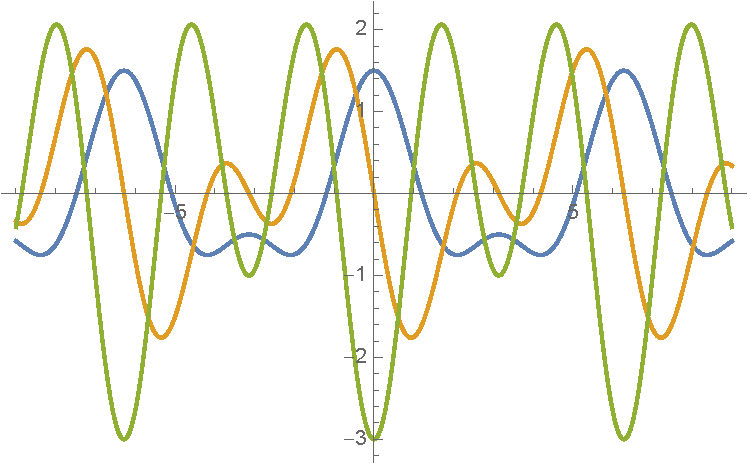
\includegraphics{./images/ch5/cosxcos2x.pdf}}
	
	{\it 蓝色、黄色和绿色分别为函数、导函数和二阶导函数的曲线}
\end{center}

\subsubsection{【综合应用】}

{\bf 例:}函数$f(x)$对满足
$$xf\,''(x)+3x[f\,'(x)]^2=1-e^{-x}$$
\begin{enumerate}[(1)]
  \setlength{\itemindent}{1cm}
  \item 若$f(x)$在$x=c\ne 0$处有极值,证明其必为极小值;
  \item 若$f(x)$在$x=0$处有极值,该极值为极大还是极小?
\end{enumerate}

{\bf 教材-习题7:}求数列$\sqrt[n]n$中最大的一项。

\begin{center}
	\resizebox{!}{5cm}{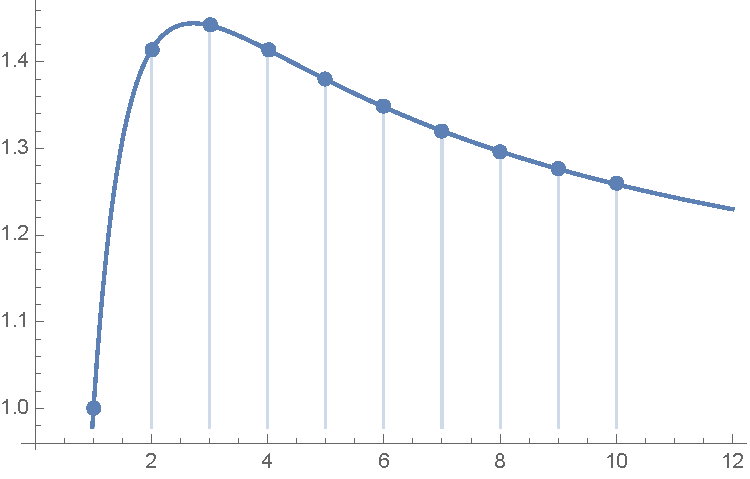
\includegraphics{./images/ch5/x1x.pdf}}
\end{center}

{\bf 例:}求$a$的取值范围,使$y=a^x$与$y=x$必相交。

{\bf 提示:}充要条件是存在$x_0>0$,满足$a^{x_0}=x_0$,也即$a$位于$g(x)=x^{x}$
的值域中。结果$a\in(0,e^{\frac1e}]$

{\bf 教材-例7:}判定方程$2^x-2x=1$有几个实根。

\begin{center}
	\resizebox{!}{5cm}{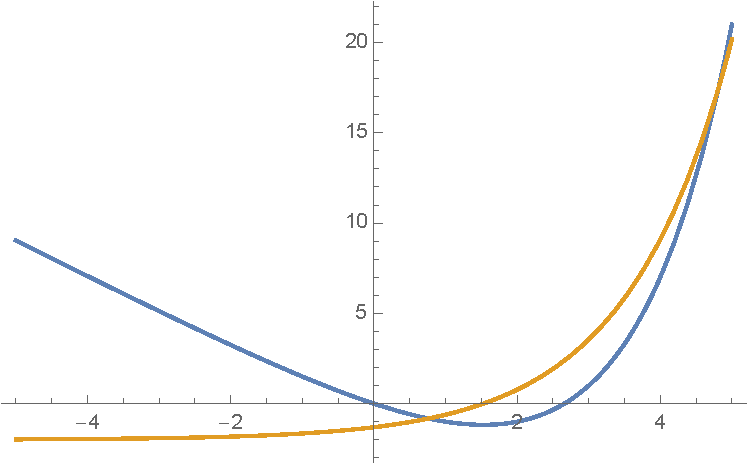
\includegraphics{./images/ch5/2x2x.pdf}}
\end{center}

{\bf 例:}已知$x>0$时,
$$kx+\df1{x^2}=1$$
有且仅有一个根,求$k$的取值范围。\ps{此类题目的叙述一定要注意逻辑表达,
既要避免过于繁琐,也要防止遗漏重要的论证}

解:令$f(x)=kx^3-x^2+1\;(x>0)$。显然原方程在$x>0$内有且仅有一个根,
当且仅当$f(x)$在$x>0$内有唯一零点。

(1)$k\leq 0$时,$f(+\infty)=-\infty$,注意到$f(0+0)=1$,
故由介值定理,$f(x)$在$x>0$上至少有一个零点。又当$x>0$时,
$f'(x)=(3kx-2)x<0$,故$f(x)$严格单调递减,从而以上零点唯一;

(2)$k>0$时,$f(+\infty)=+\infty$,令$f'(x)=0$,可得$x=\df2{3k}$
为$f(x)$的在$x>0$内的唯一驻点,又$f''\left(\df2{3k}\right)=2>0$,
故$x=\df2{3k}$为$f(x)$的最小值点。$f_{\min}=f\left(\df2{3k}\right)=1
-\df4{27k^2}$,由此可知:

若$k<\df29\sqrt3$,则$f_{\min}<0$,由介值定理,$f(x)$至少有两个零点;

若$k>\df29\sqrt3$,则$f_{\min}>0$,则当$x>0$时$f(x)>0$,无零点;

若$k=\df29\sqrt3$,则$x=\df2{3k}$为$f(x)$的唯一零点。

综上,当$k\leq 0$或$k=\df29\sqrt3$即为所求。

% {\bf 例:}$f(x)\in C[a,b]$,且在$(a,b)$内$f''(x)>0$,试讨论
% $$F(x)=\df{f(x)-f(a)}{x-a}$$
% 在$(a,b)$内的单调性。
% 
% 解:对任意$x\in(a,b)$,由Lagrange中值定理,存在$\xi\in(a,x)$,
% 使得$f(x)-f(a)=f'(\xi)(x-a)$,又由已知,$f''(x)>0$,
% 故$f'(x)$在$(a,b)$上严格单调递增,从而$f'(x)>f'(\xi)$,于是
% $$F'(x)=\df{f'(x)(x-a)+f(x)-f(a)}{(x-a)^2}=\df{f'(x)+f'(\xi)}{x-a},$$

{\bf 例:}设$a,b$均为正数,证明:$a(1-b)$和$b(1-a)$不可能同时大于$\df14$。

[提示]:令$f(x)=x(1-x)$,可求得其最大值为$\df14$。若以上两数都大于$1/4$,则
$$a(1-b)b(1-a)>\df1{16},$$
这与前述最大值的性质矛盾。

{\bf 注:}更直观的解法是,假设结论不成立,则
$$a>\df14+ab,b>\df14+ab\quad\Rightarrow\quad
ab>\left(\df14+ab\right)^2,$$
进而可得
$$\left(\df14-ab\right)^2<0,$$
出现错误,故假设不成立。

{\bf 例:}当$a$取何值时,$a^x\geq1+x$恒成立。

[提示]:两条曲线总有交点$(0,1)$,又$(a^x)''=a^x\ln^2x>0$,故$y=a^x$上凹。
要使之位于$y=x+1$上方,只需后者为其切线,由此易得$a=e$.

\begin{shaded}
{\bf 证明平均值不等式}

{\bf 例:}证明:$\df{x_1+x_2+\ldots+x_n}n\geq\sqrt[n]{x_1x_2\ldots x_n}$,
其中$x_1,x_2,\ldots,x_n$均为正数。

证:$n=2$时,设$f(x)=\df{x_1+x}2-\sqrt{x_1x}$,则
$$f'(x)=\df12\left(1-\sqrt{x_1}x\right),$$
$x=x_1$为唯一驻点,又$f''(x_1)>0$,故$f(x_1)$为最小值点。

设$n=k$时,命题成立。令
$$f(x)=\df{x_1+x_2+\ldots+x_k+x}{k+1}-\sqrt[k+1]{x_1x_2\ldots x_kx},$$
于是
$$f'(x)=\df1{k+1}\left[1-\df{{x_1x_2\ldots x_k}^{\frac1{k+1}}}
{x^{\frac k{k+1}}}\right],$$
$x_0=\sqrt[k]{x_1x_2\ldots x_k}$为唯一驻点,且$f''(x_0)>0$,故$f(x_0)$为最小值。
$$f(x_0)=\df1{k+1}(x_1+x_2+\ldots+x_k-k\sqrt[k]{x_1x_2\ldots x_k})\geq 0$$
即证。
\end{shaded}

\subsection{曲线的凹凸性}

{\bf 约定:}以下的凹凸均指“上凹”和“上凸”\ps{\b 目前的教材上对于函数的凹凸和
曲线的凹凸定义有所不同,并且刚好相反:K}

{\bf 定义5.4.1:}设函数$f(x)$在区间$I$上有定义,若对任意$x_1,x_2\in I$,
以及任意$\lambda\in[0,1]$,有
\ps{\b 直观地说,就是割线上的取值大于函数值,则称为凹,反之为凸}
$$f[\lambda x_1+(1-\lambda)x_2]\leq\lambda f(x_1)+(1-\lambda)f(x_2)$$
则称$f(x)$是区间$I$上的{\it 凹函数}。若上式中的等号严格成立,则称其为{\it 严格凹函数}。

{\bf 注:}几何特征:{\it 任意两点间的割线都不会位于两点间曲线的下方}

{\bf 定理5.4.4}(可导凹函数的充要条件)
设$f(x)$在$(a,b)$内可导,则$f(x)$为$(a,b)$内的凹函数,当且仅当:
对任意$x_1,x_2\in(a,b)$,恒有
$$f(x_2)\geq f(x_1)+f\,'(x_1)(x_2-x_1). $$
不等号严格成立时,对应于严格凹函数的情形。

{\bf 注:}{\it 任意点处的切线总位于曲线下方}

证:若$f(x)$为凹函数,对任意$x_1,x_2\in[a,b]$和任意$t\in[x_1,x_2]$,有
$$f(t)\leq\df{x_2-t}{x_2-x_1}f(x_1)+\df{t-x_1}{x_2-x_1}f(x_2)
=f(x_1)+\df{f(x_2)-f(x_1)}{x_2-x_1}(t-x_1),$$
从而
$$\df{f(t)-f(x_1)}{t-x_1}\leq\df{f(x_2)-f(x_1)}{x_2-x_1},$$
由极限的保号性,令$t\to x_1^+$,可得
$$f'(x_1)\leq\df{f(x_2)-f(x_1)}{x_2-x_1},$$
也即
$$f(x_2)\geq f(x_1)+f\,'(x_1)(x_2-x_1).$$

另一方面,由Lagrange中值定理,存在
$\xi\in(a,b)$,使得
$$\df{f(x_2)-f(x_1)}{x_2-x_1}=f'(\xi),$$
也即
$$f(x_2)=f(x_1)+f'(\xi)(x_2-x_1).$$

于是由
$$f(x_2)\geq f(x_1)+f\,'(x_1)(x_2-x_1)$$
可得
$$f'(x_1)\leq\df{f(x_2)-f(x_1)}{x_2-x_1}=f'(\xi).$$
从而
$$f(x_2)\geq f(x_1)+f'(x_1)(x_2-x_1).$$

{\bf 定理5.4.4}(充分条件)
设$f(x)$在$(a,b)$二阶可导,则
\begin{enumerate}[(1)]
  \setlength{\itemindent}{1cm}
  \item 若$f\,''(x)$恒不小于零,$f(x)$为凹函数
  \item 若$f\,''(x)$恒不大于零,$f(x)$为凸函数
\end{enumerate}

{\bf 注:}{\b{\it 拐点}即函数凹凸性发生改变的点,特别地,若函数二阶可导,则
为两侧二阶导数反号的点}\ps{拐点和极值点是“互斥”的,也即:拐点必不是极值点,反之亦然}

{\bf 讨论:}由$f''(x_0)=0$是否可以推出$x=x_0$为拐点?

答:不能!例如$y=x^3$和$y=x^4$,在$x=0$处,前者为拐点,后者是极值点!
具体可参照如下的分析方法:
\begin{center}
\begin{tabular}{c||c|c|c|c}
	\hline 
	$f(x)=x^3$ & $x<0$ & $x=0$ & $x>0$ & \\ 
	\hline 
	$f(x)$ & - & 0 & + & \\ 
	\hline 
	$f'(x)$ & + & 0 & + & 拐点\\ 
	\hline 
	$f''(x)$ & - & 0 & + & \\ 
	\hline 
	$f'''(x)$ & + & + & + & \\ 
	\hline 
	 &  &  &  &  \\ 
	\hline 
\end{tabular} 
\begin{tabular}{c||c|c|c|c}
	\hline 
	$f(x)=x^4$ & $x<0$ & $x=0$ & $x>0$ & \\ 
	\hline 
	$f(x)$ & + & 0 & + & 极小值\\ 
	\hline 
	$f'(x)$ & - & 0 & + & \\ 
	\hline 
	$f''(x)$ & + & 0 & + & \\ 
	\hline 
	$f'''(x)$ & - & 0 & + & \\ 
	\hline 
	$f^{(4)}(x)$ & + & + & + & \\ 
	\hline 
\end{tabular} 
\end{center}

{\b 事实上,$f''(x)=0$的点只能作为可能的拐点,此外,拐点也可能出现在不可导点处!}

{\bf 例:}已知多项式函数$f(x)$恰有两个极大值点和一个极小值点
\begin{enumerate}[(1)]
  \setlength{\itemindent}{1cm}
  \item 画出$f(x)$一个可能的图像
  \item 它最多有几个零点\hfill(4)
  \item 最少呢?\hfill(0)
  \item $f(x)$是奇数次还是偶数次的?\hfill(偶)
  \item 至少是多少次的?此时最多能有几个拐点?\hfill(4,4)
  \item 试给出一个它的表达式。\hfill($f(x)=(x-1)(x-2)(x-3)(x-4)$)
\end{enumerate}

\begin{shaded}
	{\it(参见: 明万元,黄香蕉,一种判断多项式函数极值点和拐点个数的简单方法,
	大学数学,2011年,第27卷第6期,161-163)
	
	http://www.doc88.com/p-0651660157725.html}
	$$P(x)=\prod_{i=1}^n(x-a_i)^{p_i}$$
	其中$a_i\in\mathbb{R}$,$p_i\in\mathbb{Z}^+\;(i=1,2,\ldots,n)$
	且$a_1<a_2<\ldots<a_n$。
	
	记$a_{i_1},\ldots,a_{i_k}$为$P(x)$的重根,$l$为其中三重根的个数。
	
	{\bf 命题:}{\bf 多项式函数的拐点、极值点判定}
	\begin{enumerate}
  	  \setlength{\itemindent}{1cm}
	  \item $P(x)$有且仅有$k+(n-1)$个驻点,包括:
	  \begin{itemize}
	    \setlength{\itemindent}{0.5cm}
	    \item $k$个重根:$a_{i_1},\ldots,a_{i_k}$
	    \item 介于两个零点之间的:$\xi_i\in(a_i,a_{i+1}),\;i=1,2,\ldots,n-1$
	  \end{itemize}
	  \item 以上所有的驻点中
	  \begin{itemize}
	    \setlength{\itemindent}{0.5cm}
	    \item 若$p_{i_j}(j=1,2,\ldots,k)$为偶数,则$a_{i_j}$为$P(x)$的极值点
	    \item 若$p_{i_j}(j=1,2,\ldots,k)$为奇数,则$a_{i_j}$为$P(x)$的拐点
	    \item $\xi_i\in(a_i,a_{i+1}),\;i=1,2,\ldots,n-1$均为极值点
	  \end{itemize}
	  \item $P''(x)$有且仅有$l+(k+n-2)$个零点
	  \begin{itemize}
	    \setlength{\itemindent}{0.5cm}
	    \item $l$个三重根
	    \item 介于每两个相邻驻点之间的:$\eta_i,\;i=1,2,\ldots,k+n-2$
	  \end{itemize}
	\end{enumerate}
	
	综上,对于前述的多项式函数,可以得出这样一些常用的{\it 判定准则}:
	\begin{enumerate}[(1)]
  	  \setlength{\itemindent}{1cm}
	  \item {\b\bf 所有二次以上的重根均为驻点,其中偶数次的为极值点,奇数次的为拐点}
	  \item {\b\bf 两个相邻零点之间有且仅有一个极值点}
	  \item {\b\bf 两个相邻驻点之间有且仅有一个拐点}
	\end{enumerate}
	
	{\bf 例:}$y=(x-1)(x-2)^2(x-3)^3$有几个极值点和拐点?
	
	\begin{center}
		\resizebox{!}{5cm}{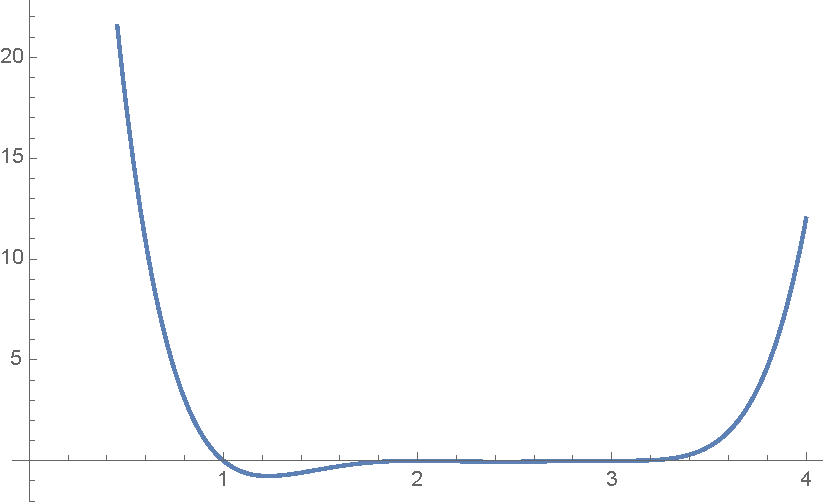
\includegraphics{./images/ch5/x123.pdf}}
	\end{center}
	
	{\bf 解:}利用前述的判定准则:
	\begin{enumerate}[(1)]
  	  \setlength{\itemindent}{1cm}
	  \item $x=2$为$2$重根,故为驻点兼极值点
	  \item $x=3$为$3$重根,故为驻点兼拐点
	  \item 在$(1,2)$和$(2,3)$中各有一个驻点兼极值点,记为$\xi_1,\xi_2$
	  \item $4$个驻点由小到大的排列为
	  $$\xi_1<2<\xi_2<3,$$
	  故在其间有且仅有$3$个拐点
	\end{enumerate}
	
	综上,该函数共有$3$个极值点,$4$个拐点。
	
	{\bf 例:}$y=2(x+1)^5(x-2)^8(x-4)^3+9$有几个极值点和拐点?
	
	\begin{center}
		\resizebox{!}{5cm}{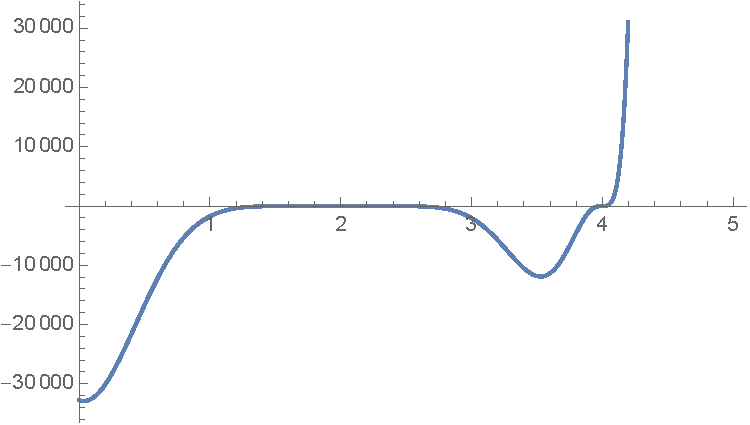
\includegraphics{./images/ch5/x124.pdf}}
	\end{center}
	
	{\bf 解:}注意到该函数和
	$$y=2(x+1)^5(x-2)^8(x-4)^3,$$
	的极值点和拐点完全相同,故我们只需研究后者的极值点和拐点个数:
	\begin{enumerate}[(1)]
  	  \setlength{\itemindent}{1cm}
	  \item $x=-1$为$5$重根,故为驻点兼拐点
	  \item $x=2$为$8$重根,故为驻点兼极值点
	  \item $x=4$为$3$重根,故为驻点兼拐点
	  \item 在$(-1,2)$和$(2,4)$中各有一个驻点兼极值点,记为$\xi_1,\xi_2$
	  \item $5$个驻点由小到大的排列为
	  $$-1<\xi_1<2<\xi_2<4,$$
	  故在其间有且仅有$4$个拐点
	\end{enumerate}
	
	综上,该函数共有$3$个极值点,$6$个拐点。
	
\end{shaded}

{\bf 推论}(教材-例11)严格凸(凹)函数的驻点为极值点。

\subsection{分析作图}

{\bf 例:}设函数$y=f(x)$具有如下性质,试作出其草图
\begin{enumerate}[(1)]
  \setlength{\itemindent}{1cm}
  \item $f(x)$在$\mathbb{R}$上连续
  \item $f(-4)=-3,f(0)=0,f(3)=2$
  \item $f'(-4)=0,f'(3)=0$,且当$x\in(-\infty,-4)\cup(-4,-3)$时,$f'(x)>0$;
  当$x\in(3,+\infty)$时,$f'(x)<0$
  \item $f''(-4)=0,f''(0)=0$,切当$x\in(-\infty,-4)\cup(0,+\infty)$时,
  $f''(x)<0$;$x\in(-4,0)$时,$f''(x)>0$
\end{enumerate}

{\bf 教材-例14:}作出函数$y=\df{x}{1+x^2}$的图形。

\begin{center}
	\resizebox{!}{5cm}{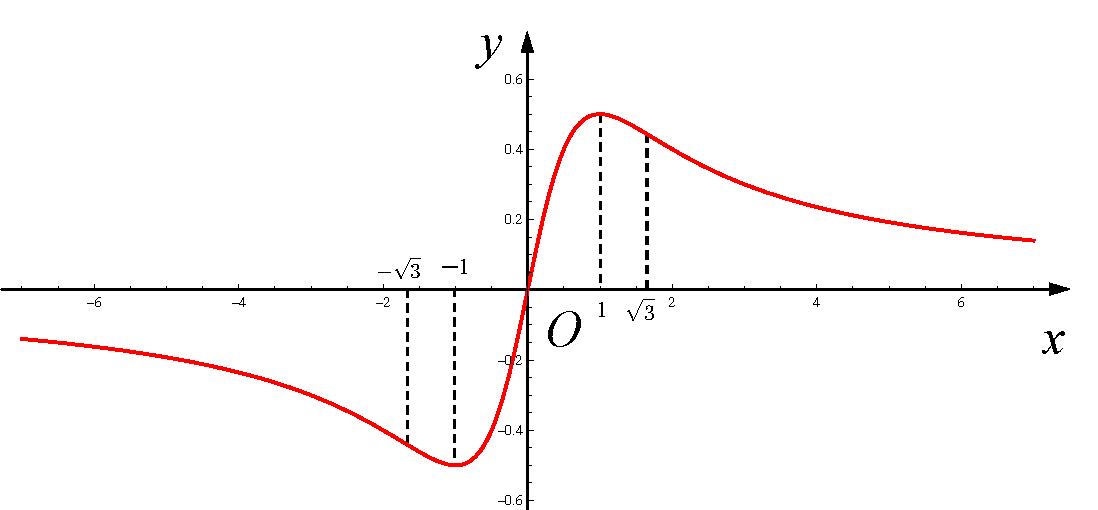
\includegraphics{./images/ch5/x1x2.pdf}}
\end{center}

\begin{shaded}
{\bf 【解题步骤】}
\begin{enumerate}[(1)]
  \setlength{\itemindent}{1cm}
  \item {\bf 分析函数一般性质:}{ 定义域、值域、奇偶性、周期性、与坐标轴的交点}
  \item {\bf 求一、二阶导函数:}{ 确定不可导点}
  \item {\bf 列表分析:}{ 单调、凸凹区间,极值点和拐点}
  \item {\bf 画出渐进线:}{ 水平、铅直和斜渐进线}
  \item {\bf 描点作图}
\end{enumerate}
\end{shaded}

{\bf 例:}函数作图:$y=xe^{1/x}$
\begin{itemize}
  \setlength{\itemindent}{1cm}
  \item 极值点:$y(1)=e$
  \item 渐近线:$y=x+1$
\end{itemize}

\begin{center}
	\resizebox{!}{7cm}{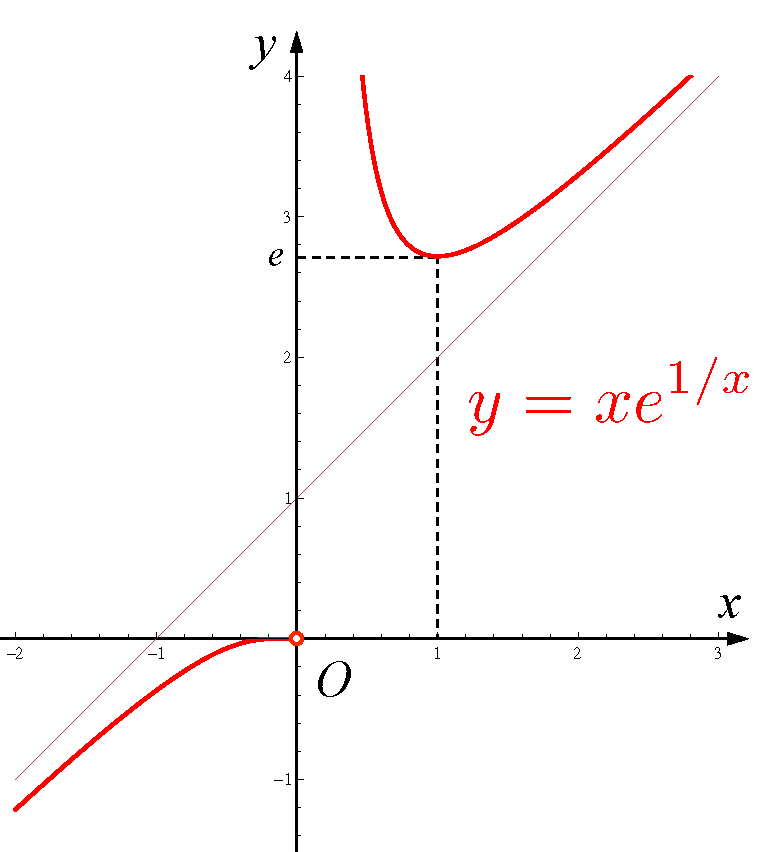
\includegraphics{./images/ch5/xe1x.pdf}}
\end{center}

\section{曲率}

% {\bf 问题:}如何刻画一条平面曲线的几何特征?
% 
% \begin{itemize}
%   \setlength{\itemindent}{1cm}
%   \item {\bf 切线斜率:}一阶导数
%   \item {\bf 凹凸性:}二阶导数
%   \item {\bf 长度:}弧微分
%   \item {\bf 弯曲程度:}曲率
% \end{itemize}

导数和二阶导数能够用于刻画曲线的倾斜程度和弯曲方向,进而可以研究曲线的极值、最值、
拐点等重要的几何特征。本节要介绍的弧微分和曲率是对以上刻画方式的补充,前者用于
计算曲线的长度,后者则是曲线弯曲程度的度量(量化)。特别要指出的是,这两个重要
的概念是“纯几何”的,也就是说其计算所得到的结果(弧长和曲率)都和坐标的选取无关!

\subsection{弧微分}

曲线$y=f(x)$的弧长关于自变量$x$的微分\ps{严谨的推导过程请参考同济教材第三章第七节}
$$\d s=\sqrt{1+(y')^2}\d x =\sqrt{(\d x)^2+(\d y)^2}$$ 
\begin{itemize}
  \setlength{\itemindent}{1cm}
  \item 参数方程形式 
  $$\d s=\sqrt{[x'(t)]^2+[y'(t)]^2}\d t$$ 
  \vspace{-3ex}
  \item 极坐标形式 
  $$\d s=\sqrt{\rho^2(\theta)+[\rho'(\theta)]^2}\d\theta$$
\end{itemize}
不难想到,如果给定积分的区间,对弧微分进行积分,可以得到对应的弧长(曲线长度)。

% {\bf 例:}求$y=x^2$对应于$x\in[0,1]$的曲线长度。

\subsection{曲率}

\begin{center}
	\resizebox{!}{7cm}{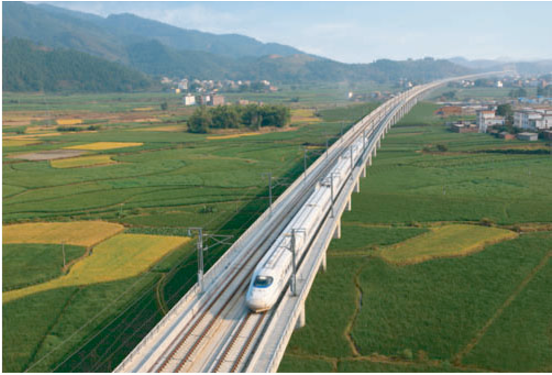
\includegraphics{./images/ch5/rw1.pdf}}
	
	{\it 铁路设计中的问题:列车从直线轨道进入圆弧轨道时,在转换的瞬间,
	
	离心力由零变为一个常数,如果车速较快,会车体和乘客产生很大的冲击。
	
	能否/如何通过更合理的设计,减缓冲击,保证列车运行的安全、舒适?}
\end{center}

\subsubsection{【概念】}

{\bf 问题:}如何刻画曲线的弯曲程度?

\begin{center}
	\resizebox{!}{5.5cm}{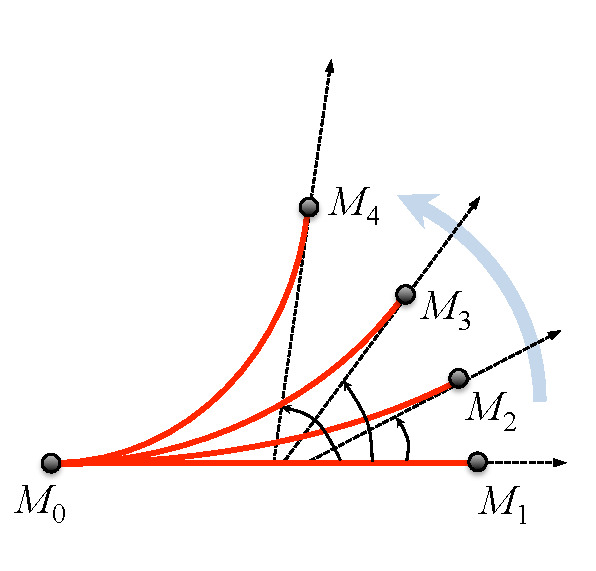
\includegraphics{./images/ch5/curves/c101.pdf}}\quad
	\resizebox{!}{5.5cm}{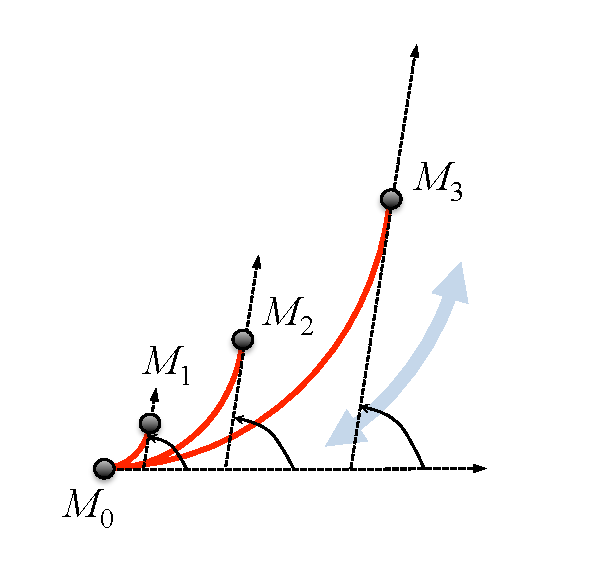
\includegraphics{./images/ch5/curves/c201.pdf}}
\end{center}

\begin{itemize}
  \setlength{\itemindent}{1cm}
  \item 长度相同的曲线,切线转角越大弯曲程度越大
  \item 切线转角相同的曲线,弧长越短弯曲程度越大
\end{itemize}

{\it 曲线的弯曲程度与切线的转角成正比,与弧长成反比}

{\bf 定义5.5.1:}设曲线$C$光滑且可求长度。 从其上一点$M_0$出发,
到另一点$M$的弧长为$\Delta s$,切线转角为$\Delta\alpha$。
 若极限$\lim\limits_{\Delta s\to
0}\left|\df{\Delta\alpha}{\Delta s}\right|$存在,
则称之为{\it 曲线$C$在$M_0$处的曲率:}

$${K=\lim\limits_{\Delta s\to
0}\left|\df{\Delta\alpha}{\Delta s}\right|
=\left|\df{\d\alpha}{\d s}\right|}$$ 

{\bf 曲率:}在曲线上某一点处的切线转角关于弧长的变化率

% $$K=\df{|y''|}{(1+(y')^2)^{\frac32}}$$

设$y=f(x)$在$x_0$的某邻域内二阶可导,则
{\b $$K=\left|\df{\d\alpha}{\d s}\right|
 =\df{|y''_{xx}|}{[1+(y'_x)^2]^{3/2}}$$}
 
{\bf 教材-例2:}求直线与圆的曲率。

{\bf 例:}求椭圆$x=3\cos t,y=2\sin t\,(0\leq t\leq 2\pi)$
上任意点处的曲率,并指出其中曲率最大的点。

\begin{center}
	\resizebox{!}{4.5cm}{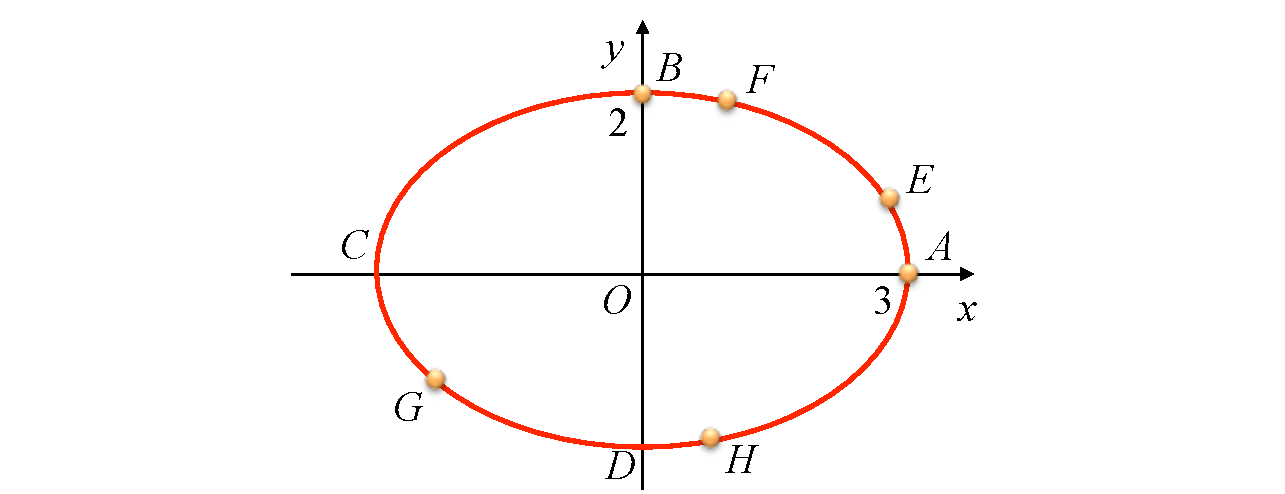
\includegraphics{./images/ch5/ec/newEC/ec01.pdf}}
\end{center}

{\bf 注:} {参数方程下的曲率公式}
$${K=\df{|x'_ty''_{tt}-x''_{tt}y'_t|}
{\{[x'_t]^2+[y'_t]^2\}^{3/2}}}$$

极坐标下的曲率公式
$$K=\df{|\rho^2+2(\rho')^2-2\rho\rho''|}{[\rho^2+(\rho')^2]^{3/2}}$$

{\bf 思考:}如何给出极坐标下的曲率公式?

\subsubsection{【曲率圆与曲率的应用】}

{\it 曲率圆:}与给定曲线在凹侧相切,且曲率相同的圆
\ps{曲率圆的圆心称为{\it 曲率中心}}

{\bf 定理:}曲率圆与给定曲线二阶相切。

{\bf 思考:}{\b 与已知曲线在给定点处二阶相切的圆一定是其曲率圆吗?(${\bm{\surd}}$)}

{\bf 例:}求曲率圆的方程

\begin{center}
	\resizebox{!}{5cm}{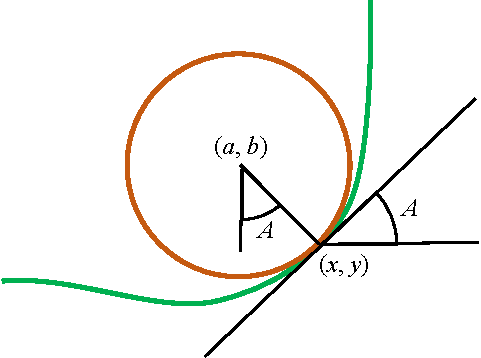
\includegraphics{./images/ch5/curveSphere.pdf}}
\end{center}

[提示]:如图,设曲率圆的圆心为$(a,b)$,$(x,y)$处的导数和二阶导数记为$y',y''$,
显然曲率半径$R=\df1K=\df{[1+(y')^2]^{3/2}}{|y''|}$,为了保持和曲线的凹向一致,
我们将曲率半径定义为有方向的$R=\df{[1+(y')^2]^{3/2}}{y''}$\ps{凹侧的半径为正,
凸侧为负!}。记$(x,y)$处的切线与$x$轴夹角为$A$,则
\begin{align}
	a&=x-R\sin A=x-\df{[1+(y')^2]^{3/2}}{y''}\df{y'}{[1+(y')^2]^{1/2}}
	=x-\df{y'[1+(y')^2]}{y''}\notag\\
	b&=y+R\cos A=y+\df{[1+(y')^2]^{3/2}}{y''}\df1{[1+(y')^2]^{1/2}}
	=y+\df{1+(y')^2}{y''}\notag
\end{align}

\begin{center}
	\resizebox{!}{5.5cm}{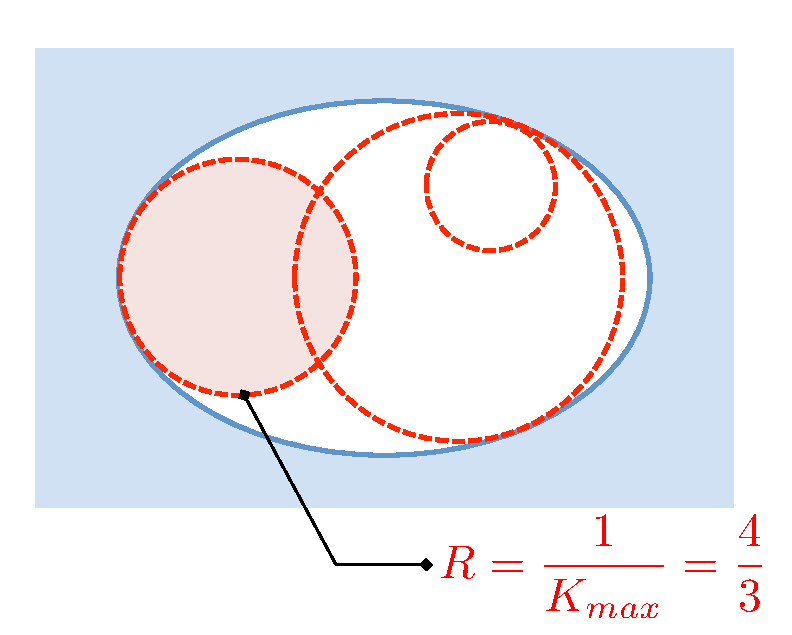
\includegraphics{./images/ch5/SE/S01.pdf}}
\end{center}

{\bf 例}(加工问题)已知某工件内侧的截痕曲线为椭圆$\df{x^2}9+\df{y^2}4=1$,
若用圆形砂轮对其进行打磨,问该如何选择砂轮的尺寸?

{\bf 注:}利用砂轮磨削一般工件的内表面时,砂轮的半径不应超过工件内表面
的截线上各点处的曲率半径的最小值

{\bf 定律:}质量为$m$的质点以速度$v$通过光滑曲线上一点,所受离心力为
$$F=\df{mv^2}{R},$$
其中$R$为曲线在该点处的曲率半径。

\begin{center}
	\resizebox{!}{3cm}{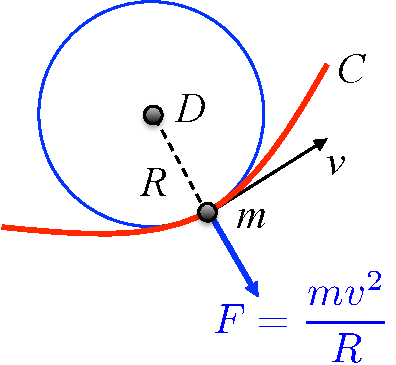
\includegraphics{./images/ch5/flip.pdf}}
\end{center}

{\bf 例:}$\Gamma_1$为射线$y=0,x\leq0$,$\Gamma_2$为椭圆$\df{4(x-2)^2}9+y^2=1$。
使找出一条次数尽可能低的多项式函数曲线$\Gamma_2$,连接$(0,0)$和$(2,1)$,使得最终
完整的曲线曲率连续。

{\bf 提示:}$\Gamma_2$在$(2,1)$处的曲率为$-\df49$。
设新的曲线为$\Gamma_3:y=y(x)$,显然
$$y(0)=0,\;y'(0)=0,\;y''(0)=0,$$
$$y(2)=1,\;y'(2)=0,\;y''(2)=-\df49$$
六个条件,意味着至少需要一个$5$次多项式。考虑到$y(0)=y'(0)=y''(0)=0$,
可设$y=ax^3+bx^4+cx^5$,于是
$$
\left\{
\begin{array}{l}
1=8a+16b+32c\\
0=12a+32b+80c\\
-\df49=12a+48b+160c
\end{array}
\right.
$$
行列式非零,方程组解唯一。

\subsubsection{【铁路中的缓和曲线】}

\begin{center}
	\resizebox{!}{9cm}{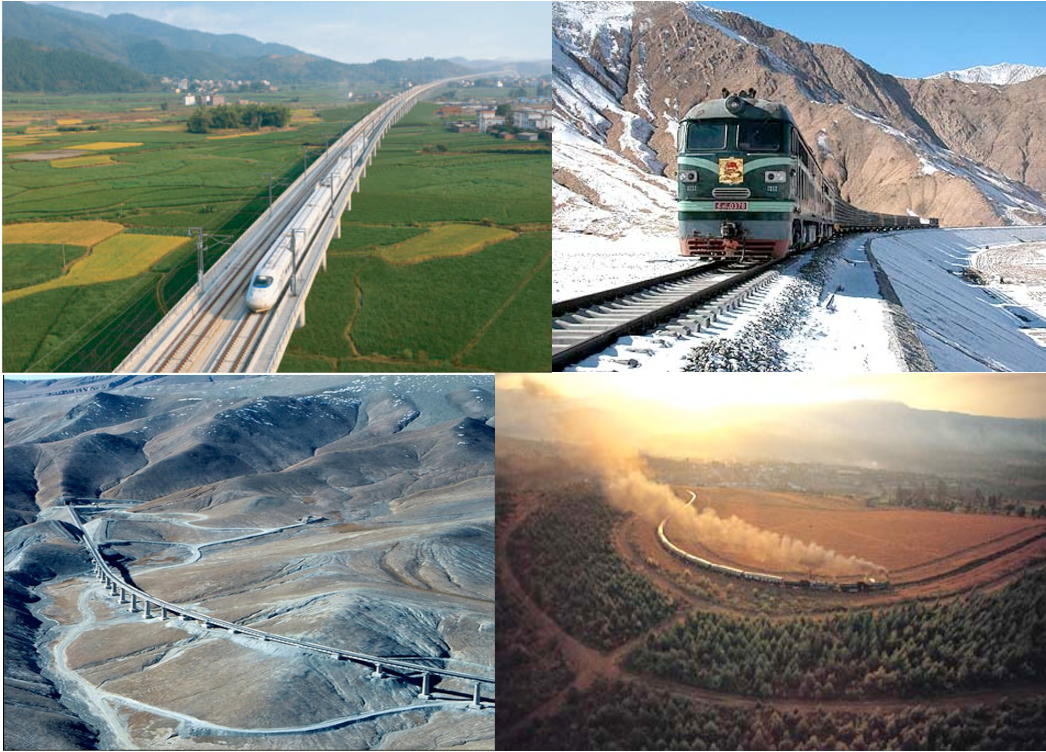
\includegraphics{./images/ch5/railway.pdf}}
\end{center}

{\bf 设计要求:}为了确保列车行驶安全,尽可能保证列车运行时所受离心力的平稳变化

{\bf 常用的缓和曲线:}三次多项式、渐开螺旋线、双纽线、\ldots

{\bf 例:}如图,列车匀速行进,经过一段直线轨道后,将进入半径为$R$的圆弧轨道。为
尽量减少列车行驶中所受的离心力冲击,试确定一个三次多项式函数实现两段轨道的连接。

\begin{center}
	\resizebox{!}{5.2cm}{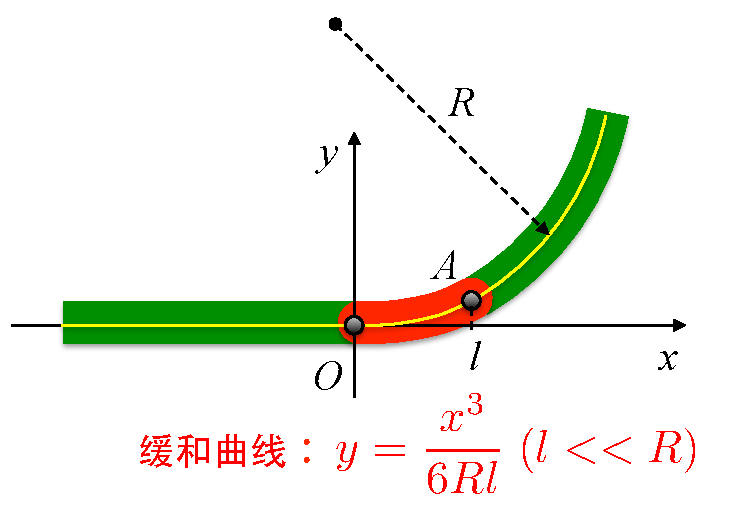
\includegraphics{./images/ch5/rc01.pdf}}
\end{center}

\begin{itemize}
  \item 匀速行驶$v=108km/h$
  \item 列车重量$m=500t$
  \item 圆弧半径$R=1000m$
  \item 缓和曲线长$l=90m$
\end{itemize}

\begin{center}
	\resizebox{!}{4cm}{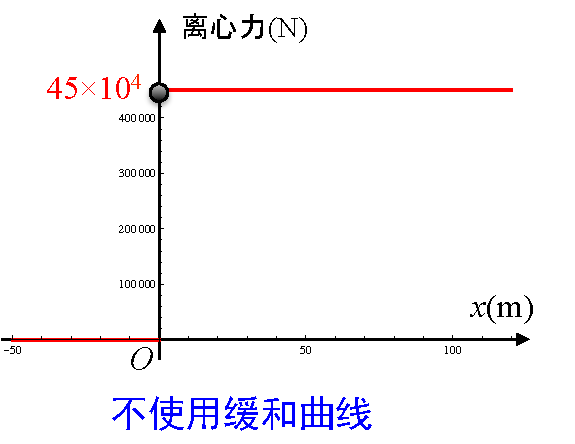
\includegraphics{./images/ch5/f01.pdf}}\quad
	\resizebox{!}{4cm}{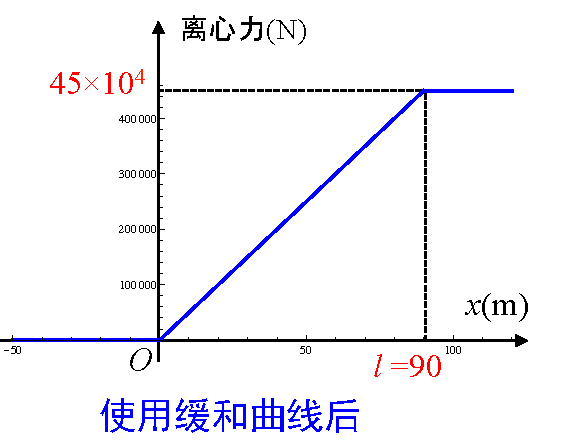
\includegraphics{./images/ch5/f02.pdf}}
\end{center}

类似的问题广泛存在于高速公路、过山车,甚至是飞行器表面的设计中。

\section{小结}

导数为我们提供了研究函数和平面曲线的新的工具。Newton正是因为发明了{\it 流数法
\ps{导数的前身}},才从Kepler三定律推导出了万有引力定律。

本章的内容包含两个大的方面:一是对函数几何形态的研究,涉及:{\it 单调性、最值、极值、
凹凸性、弧长、曲率等}多个方面,由此最终可以对给定的函数给出一个相对
全面的几何刻画,其中很多是在大学之前所不曾接触的;二是{\it 中值定理与Taylor公式},特别是
后者,可以说是微分学中的集大成者,其中蕴含了几乎所有的微分学理论与技巧,从Rolle定理、
Lagrange中值定理、Cauchy中值定理到Taylor中值定理,以及L'Hospital法则,其
内在的统一是学习中需要把握的重点。

在极值、最值、凹凸性等问题中,涉及一些相近而不同的概念,例如:极值点、最值点、拐点、
驻点等,这些概念既相互联系,又有重要的区别,琢磨弄懂它们的异同,能够结合实例有效
地加以区分和应用,是学习的关键。当然,既然是讨论几何问题,对于几何意义和几何特征
的正确把握也是非常重要的。

中值定理的证明问题是本章的难点,从结论出发,构造辅助函数,再验证条件应用中值定理,
是解题的一般思路,但有时如何将结果转换成可以还原的形式,会是相当大的挑战,
为此,有必要掌握一些特定形式(例如:$f'(\xi)+\lambda f(x)$)所对应的辅助函数。
此外,本章两个部分的内容本身并不是相互独立的,事实上,很多结论的推导和证明都需要
同时应用两个部分的结果,特别是从几何上看,中值定理也通常有自身明确的含义,而能够
结合几何意义解决中值问题,可以说才是本章解题的最高境界。

最后,提醒一句,不要迷恋Taylor公式,还是那句话,万能工具虽然万能,但往往不是
效率最高和用起来最简单的一个。

\newpage

\section*{课后作业}
\addcontentsline{toc}{section}{课后作业}

{\bf 【必作题】}

\begin{itemize}
  \item 习题5.1:6(2,4),9,11,12,14
  \item 习题5.2:3,6,9,10,12,14,16
  \item 习题5.3:1,2,4,5,6,10,12,13,14
  \item 习题5.4:6(2,4),7,9,11,13,14(3)
  \item 习题5.5:3,5,6,7,10
\end{itemize}

\bigskip

\hrule

\bigskip
\bigskip

{\bf 【思考题】}

\begin{itemize}
  \item 习题5.1:7,13
  \item 习题5.2:4,5,7,8,11,13,15,17,18,19
  \item 习题5.3:3,8,9,16,17
  \item 计算如下极限
  	\begin{enumerate}
	  \item $\limx{0}\df{e^x-e^{-x}-2x}{x-\sin x}$ 
	  \item $\limx{0}\df{e^{-1/x^2}}{x^{100}}$ 
	  \item $\limx{a}\df{x^a-a^x}{x^x-a^a}\;(a>0)$ 
	  \item $\limx{0}\left(\df{a^x+b^x+c^x}{3}\right)^{1/x}$ 
	  \item $\limn\sqrt{n}(\sqrt[n]{n}-1)$ 
	  \item $\limn\left(n\sin\df{1}{n}\right)^{n^2}$
	\end{enumerate}	
  \item 习题5.4:4,5,8,12,15-21
  \item 习题5.5:15
\end{itemize}

\newpage

\section*{补充例题}
% \addcontentsline{toc}{section}{补充例题}

{\bf 例:}$a$取何值时,$f(x)=2x^3-9x^2+12-a$恰有两个零点(B)

A)$2$\quad B)$4$\quad C)$6$\quad D)$8$

分析:$f'(x)=6(x-2)(x-1)$,$x=1,2$为极值点,若$f(1)$或$f(2)$为零,即有结论成立。

{\bf 例:}$f(x)$在$x>0$二阶可导,$f''(x)>0$,令$u_n=f(n)\;(n\in\mathbb{Z}_+)$,
则(D)
\begin{enumerate}[A)]
  \setlength{\itemindent}{1cm}
  \item 若$u_1>u_2$,则$\{u_n\}$必收敛;
  \item 若$u_1>u_2$,则$\{u_n\}$必发散;
  \item 若$u_1<u_2$,则$\{u_n\}$必收敛;
  \item 若$u_1<u_2$,则$\{u_n\}$必发散;
\end{enumerate}

分析:$u_1<u_2$,则$\exists\xi\in(1,2)$,$f'(\xi)>0$,
又$x>\xi$时,$f'(x)>f'(\xi)$,故
$$f(x)>f(\xi)+f'(\xi)(x-\xi)\to+\infty\;(x\to+\infty)$$

{\bf 例:}$f(x)=|x(1-x)|$,则$x=0$(C)
\begin{enumerate}[A)]
  \setlength{\itemindent}{1cm}
  \item 是极值点,但不是拐点
  \item 不是极值点,但是拐点
  \item 是极值点,也是拐点
  \item 不是极值点,也不是拐点
\end{enumerate}

{\bf 例:}求$y=\df1x+\ln(1+e^x)$的渐近线

分析:$x=0,y=x,y=0$

{\bf 例:}$f(x)$二阶导数连续,$f'(0)=0$,$\limx{0}\df{f''(x)}{|x|}=1$,
则(B)
\begin{enumerate}[A)]
  \setlength{\itemindent}{1cm}
  \item $f(0)$是$f(x)$的极大值点
  \item $f(0)$是$f(x)$的极小值点
  \item $f(0)$是$f(x)$的拐点
  \item $f(0)$不是极值点,也不是拐点
\end{enumerate}

{\bf 例:}$f(x)\in C(a,b)$,$f(a)=f(b)=0$,$f'(a)f'(b)>0$,
证明:$f(x)$在$(a,b)$内至少有一个零点。

{\bf 例:}$f(x)$在$[a,b]$可导,且$f'(a)f'(b)<0$,证明:存在$\xi\in(a,b)$,
使得$f'(\xi)=0$.

{\bf 例:}证明:$(x^2-1)\ln x\geq(x-1)^2,(x>0)$

分析:令$f(x)=\ln x-\df{x-1}{x+1}$,则$f'(x)>0,(x>0)$

{\bf 例:}证明:$\df{e^a-e^b}{b-a}<\df{e^a+e^b}2,\;(a\ne b)$

分析:不妨$a<b$,令$f(x)=\df{e^a+e^x}2-\df{e^a-e^x}{b-a}$

{\bf 例:}$e<a<b<e^2$,证明:$\ln^2b-\ln^2a>\df4{e^2}(b-a)$

分析:$f(x)=\ln^2x$,由Lagrange中值定理,存在$\xi\in(a,b)$,
$$\df{\ln^2b-\ln^2a}{b-a}=\df{2\ln\xi}{\xi},$$
再证明$\df{\ln\xi}{\xi}>\df2{e^2},\xi\in(a,b)\in(e,e^2)$

{\bf 例:}$a>1$,$x\in[0,1]$,证明:
$$\df1{2^{a-1}}\leq x^a+(1-x)^a\leq 1$$

分析:令$f(x)=x^a+(1-x)^a$

{\bf 例:}证明$x>0,y>0$时,$xy\leq x\ln x+e^{y-1}$

分析:证明$f(x)=\ln x+\df{e^{y-1}}y$最小值大于$y$即可。

{\bf 例:}$f_n(x)=\sin x+\sin^2x+\ldots+\sin^nx$,证明:
\begin{enumerate}[1)]
  \setlength{\itemindent}{1cm}
  \item $f_n(x)=1$在$\left(\df{\pi}6,\df{\pi}2\right)$内有且仅有一个根
  \item 设$x_n\in\left(\df{\pi}6,\df{\pi}3\right)$是以上的根,则$\limn x_n=\df{\pi}6$
\end{enumerate}

分析:1)介值定理,且$f(x)$严格单增;

2)$f_n\left(\df{\pi}{6}\right)=1-\df1{2^n}$,
$f'_n\left(\df{\pi}{6}\right)>\sqrt
3>1$,$n$充分大时 $$f'_n\left(\df{\pi}{6}+\df1{2^{n-1}}\right)
=f_n\left(\df{\pi}{6}\right)+f'_n\left(\df{\pi}{6}\right)\df1{2^{n-1}}
+\circ\left(\df1{2^{n-1}}\right)>1+\df1{2^n},$$
故$x_n\in\left(\df{\pi}{6},\df{\pi}{6}+\df1{2^{n-1}}\right)$

{\bf 例:}证明$x>0$时,$\df1{x(x+1)}>\ln^2(1+1/x)$

分析:令$y=1/x$,证明
$$y-\sqrt{1+y}\ln(1+y)>0$$

{\bf 例:}证明:$\df{\tan x}x>\df x{\sin x}$,$x\in(0,\pi/2)$

分析:$f(x)=\sin x\tan x-x^2$,$f(0)=f'(0)=f''(0)=0$,$f'''(x)>0$

{\bf 例:}$t\in[0,x]$,证明:$e^{-t}\geq\left(1-\df tx\right)^x$

分析:$t=0,x$时,显然成立。此外,设$f(x)=x\ln\left(1-\df tx\right)+t$,
则$\limx{+\infty}=0$,证明$f'(x)=\ln\left(1-\df tx\right)+\df t{x-t}>0$即可。

$u>0$时,$u>\ln(1+x)$,故
$$\df t{t-x}>\ln\left(1+\df t{x-t}\right)=-\ln\left(1-\df tx\right)$$

{\bf 例:}比较$\pi^e$和$e^{\pi}$

分析:令$f(x)=x-e\ln x$

{\bf 例:}$f(x),g(x)$均在$[a,b]$内二阶可导且存在相同的最大值,$f(a)=g(a)$,
$f(b)=g(b)$,则存在$\xi\in(a,b)$,$f''(\xi)=0$。

{\bf 例:}$f(x)$在$[0,1]$上二阶可导,$f(0)=0,f(1)=1$,$f''(0)<0$,则
$\df{f(x)}x$在$(0,1]$上严格单调递减

{\bf 例:}$y=f(x)\in C^2(-1,1)$,$f''(x)\ne 0$,则:
\begin{enumerate}[1)]
  \setlength{\itemindent}{1cm}
  \item 对于任意$x\in(-,1),x\ne 0$,存在唯一的$\theta(x)\in(0,1)$,使得
  $f(x)=f(0)+xf'(\theta(x)x)$成立
  \item $\limx{0}\theta(x)=\df12$
\end{enumerate}

分析:1)Lagrange中值定理,若$\theta(x)$不唯一,则与$f''(x)\ne 0$矛盾;

2)
$$\df{f'(\theta(x)x)-f'(0)}{x}=\df{f(x)-f(0)-xf'(0)}{x^2}\to\df12f''(0),(x\to0)$$
$$\df{f'(\theta(x)x)-f'(0)}{x}=f''(0)\limx{0}\theta(x)$$

\newpage

\section*{习题5.3参考解答}
\addcontentsline{toc}{section}{习题5.3参考解答}

1. 将$f(x)=x^3+3x^2-2x+4$在$x_0=-1$处展开成Taylor公式。

解:因为
$$f(x)=[(x+1)-1]^3+3[(x+1)-2]^2-2[(x+1)-1]+4
=8-5(x+1)+(x+1)^3,$$
故$f(x)$在$x_0=-1$处的各阶带Peano余项的Taylor公式依次为
\begin{align}
	P_1(x)&=8-5(x+1)+\circ(x+1)\notag\\
	P_2(x)&=8-5(x+1)+\circ((x+1)^2)\notag\\
	P_3(x)&=8-5(x+1)+(x+1)^3+\circ((x+1)^3)\notag\\
	P_k(x)&=8-5(x+1)+(x+1)^3+\circ((x+1)^k),\;k>3.\notag
\end{align}

\bigskip

2. 已知$f(x)$是四次多项式,且$f(2)=-1,f'(2)=0,f''(2)=-2,f'''(2)=-12,
f^{(4)}(x)=24$,求$f(-1)$.

解:由已知,$f(x)$在$x=2$处的Taylor多项式的各阶系数依次为
\begin{align}
	a_0&=f(2)=-1\notag\\
	a_1&={f'(2)}=0\notag\\
	a_2&=\df{f''(2)}2=-1\notag\\
	a_3&=\df{f'''(2)}{3!}=-2\notag\\
	a_4&=\df{f^{(4)}(2)}{4!}=1\notag
\end{align}
因为$f(x)$为四阶多项式,故其四阶Taylor多项式即为其自身,从而
$$f(x)=-1-(x-2)^2-2(x-2)^3+(x-2)^4,$$
由此易得$f(-1)=125$.

\bigskip

4. 写出下列函数带Peano余项的Maclaurin公式

(1) $f(x)=\ln(2+x)$
\begin{align}
	\ln(2+x)&=\ln2+\ln\left(1+\df x2\right)\notag\\
	&=\ln2+\sum\limits_{k=1}^n\df{(-1)^{k-1}}{k}\left(
	\df{x}2\right)^k+\circ\left(\left(\df x2\right)^n\right)\notag\\
	&=\ln2+\sum\limits_{k=1}^n\df{(-1)^{k-1}}{2^kk}x^k+\circ(x^n)\notag
\end{align}

(2) $f(x)=e^{-x^2}$
\begin{align}
	e^{-x^2}&=\sum\limits_{k=0}^n\df{(-x^2)^k}{k!}+\circ((-x^2)^n)\notag\\
	&=\sum\limits_{k=0}^n\df{(-1)^k}{k!}x^{2k}+\circ(x^{2n})\notag
\end{align}

(3) $f(x)=x\sin x$
\begin{align}
	x\sin x&=x\left[\sum\limits_{k=0}^n\df{(-1)^k}{(2k+1)!}x^{2k+1}
	+\circ(x^{2n+1})\right]\notag\\
	&=\sum\limits_{k=0}^n\df{(-1)^k}{(2k+1)!}x^{2k+2}
	+\circ(x^{2n+2})\notag
\end{align}

(4) $f(x)=\df{x^2}{1+x}$
\begin{align}
	\df{x^2}{1+x}&=x^2\left[\sum\limits_{k=0}^n(-x)^k
	+\circ((-x)^n)\right]\notag\\
	&=\sum\limits_{k=0}^n(-1)^kx^{k+2}+\circ(x^{n+2})\notag
\end{align}

(5) $f(x)=\df1{\sqrt{1-x^2}}$
\begin{align*}
	\df1{\sqrt{1-x^2}}&=[1+(-x^2)]^{-\frac12}
	=\sum\limits_{k=0}^n\left(\begin{array}{c}
	-\frac12 \\ k\end{array}\right)
	(-x^2)^k+\circ((-x^2)^n) \\
	&=\sum\limits_{k=0}^n\left(\begin{array}{c}
	-\frac12 \\ k\end{array}\right)
	(-1)^kx^{2k}+\circ(x^{2n})
	=\sum\limits_{k=0}^n\frac{(2k-1)!!}{2^kk!}x^{2k}
	+\circ(x^{2n})
\end{align*}

(6) $f(x)=\cos^2x$
\begin{align}
	\cos^2x&=\df{1+\cos2x}2\notag\\
	&=\df12+\df12\left[\sum\limits_{k=0}^n\df{(-1)^k}{(2k)!}(2x)^{2k}
	+\circ(x^{2n})\right]\notag\\
	&=\df12+\sum\limits_{k=0}^n\df{(-1)^k2^{2k-1}}{(2k)!}(x)^{2k}
	+\circ(x^{2n})\notag
\end{align}

\bigskip

5. 求函数$f(x)=\df1x$在$x=-1$处带Lagrange余项的$n$阶Taylor公式

解:$f^{(n)}(x)=\df{(-1)^nn!}{x^{n+1}}$,故存在$\xi$介于$x$和$-1$之间,使得
\begin{align}
	f(x)&=\df1{-1+(x+1)}=-\df1{1-(x+1)}\notag\\
	&=-\sum\limits_{k=0}^n(x+1)^k
	+\df{(-1)^{n+1}(n+1)!}{\xi^{n+2}}(x+1)^{n+1},\notag
\end{align}
即为所求。

\bigskip

6. 将函数$f(x)=\ln x$按$x-2$的幂展开成带Peano余项的$n$阶Taylor公式。

解:
\begin{align}
	f(x)&=\ln(2+(x-2))=\ln2+\ln\left(1+\df{x-2}2\right)\notag\\
	&=\ln2+\sum\limits_{k=1}^n\df{(-1)^{k-1}}{k}
	\left(\df{x-2}2\right)^k+\circ\left(\left(\df{x-2}2\right)^n\right)\notag\\
	&=\ln2+\sum\limits_{k=1}^n\df{(-1)^{k-1}}{2^kk}
	(x-2)^k+\circ((x-2)^n)\notag
\end{align}

\bigskip

10. 利用Taylor公式求下列极限

(1)
\begin{align}
	\limx0\df{xe^x-\ln(1+x)}{x^2}
	&=\limx0\df{x+x^2+\circ(x^2)-[x-\frac{x^2}2+\circ(x^2)]}{x^2}\notag\\
	&=\df32+\limx0\circ(1)=\df32\notag
\end{align}

(2)
\begin{align}
	\limx{+\infty}&\left[\left(x^3-x^2+\df x2\right)e^{\frac1x}
	-\sqrt{x^6+1}\right]
	\xlongequal{u=1/x}\lim\limits_{u\to0^+}
	\df{(1-u+2u^2)e^u-\sqrt{1+u^6}}{u^3}\notag\\
	&=\lim\limits_{u\to0^+}\df{\left(1-u+\frac{u^2}2\right)
	\left(1+u+\frac{u^2}2+\frac{u^3}6+\circ(x^3)\right)
	-[1+\frac12u^6+\circ(u^6)]}{u^3}\notag\\
	&=\lim\limits_{u\to0^+}\df{\frac{u^3}6+\circ(u^3)}{u^3}
	=\df16+\lim\limits_{u\to0^+}\circ(1)=\df16\notag
\end{align}

(3)
\begin{align}
	\limx{+\infty}&\left[x-x^2\ln\left(1+\df1x\right)\right]
	\xlongequal{u=1/x}\lim\limits_{u\to0^+}
	\df{u-\ln(1+u)}{u^2}\notag\\
	&=\lim\limits_{u\to0^+}\df{u-[u-\frac{u^2}2+\circ(u^2)]}{u^2}
	=\df12+\lim\limits_{u\to0^+}\circ(1)=\df12\notag
\end{align}

(4)
\begin{align}
	\limx0&\df{\frac{x^2}2+1-\sqrt{1+x^2}}{x^2\sin x^2}
	=\limx0\df{\frac{x^2}2+1-[1+\frac12x^2-\frac18x^4+\circ(x^4)]}{x^4}\notag\\
	&=\df18+\limx0\circ(1)=\df18\notag
\end{align}

\bigskip

12. 常数$a,b$为何值时,成立$\limx0\left[\df{\ln(1+2x)}{x}+a
+\df bx\right]=0$?

解:
$$\df{\ln(1+2x)+ax+b}{x}=\df{2x+\circ(x)+ax+b}x=(a+2)+\circ(1)+\df bx,$$
显然以上函数若当$x\to0$时极限存在,则必有$b=0$;又由极限值为$0$,可知$a+2=0$,
故$a=-2$。

\bigskip

13. 设$f(x)$在$x=0$附近二次可导,且
$$\limx0\left(\df{\sin x}{x^3}+\df{f(x)}{x^2}\right)=0,$$
(1) 求$f(0).f'(0),f''(0)$;(2)计算$\limx0\df{1+f(x)}{x^2}$.

解:由已知
$$0=\limx0\left(\df{\sin x}{x^3}+\df{f(x)}{x^2}\right)
=\limx0\df{x-\frac{x^3}6+\circ(x^3)+xf(x)}{x^3}
=\limx0\df{1+f(x)}{x^2}-\df16,$$
故$\limx0\df{1+f(x)}{x^2}=\df16$。
$$\limx0[1+f(x)]=\limx0\df{1+f(x)}{x^2}\limx0x^2=0,$$
从而$f(0)=\limx0f(x)=-1$。又
$$f'(0)=\limx0\df{f(x)-f(0)}{x-0}=\limx0\df{f(x)+1}{x}
=\limx0\df{f(x)+1}{x^2}\limx0x=0,$$
于是由Taylor公式,可设$f(x)=-1+\df{f''(0)}2x^2+\circ(x^2)$,进而
$$\df16=\limx0\df{1+f(x)}{x^2}=\df{f''(0)}2+\limx0\circ(1)
=\df{f''(0)}2\quad\Rightarrow\quad f''(0)=\df13.$$
以上即为所求。

\bigskip

14. 设函数$f(x)$在$[0,1]$上二次可导,且$f(0)=f(1)$,$|f''(x)|\leq2$,
证明:$x\in[0,1]$时,有$|f'(x)|\leq 1$.

证:对任意$x\in[0,1]$,由Taylor公式,存在$\xi_1\in(0,x),\xi_2\in(x,1)$,
使得
$$f(0)=f(x)+f'(x)(-x)+\df{f''(\xi_1)}2x^2,$$
$$f(2)=f(x)+f'(x)(1-x)+\df{f''(\xi_2)}2(1-x)^2,$$
以上两式相减,整理后可得
$$f'(x)=-\df12\left[f''(\xi_2)(1-x)^2-f''(\xi_1)x^2\right],$$
从而
\begin{align}
	|f'(x)|&=\df12\left|f''(\xi_2)(1-x)^2-f''(\xi_1)x^2\right|\notag\\
	&\leq\df12\left[|f''(\xi_2)|(1-x)^2+|f''(\xi_1)|x^2\right]\notag\\
	&\leq(1-x)^2+x^2\notag
\end{align}
注意到,当$x\in[0,1]$时,$(1-x)^2+x^2$最大值为$1$,故由上式可得$|f'(x)|\leq1$,
即证。